% ============================================================
%  CAAS — Final Project Report
%  AT82.9002 Data Engineering and MLOps, AIT
%  Supanut Kompayak (st126055) · Shuvam Shrestha (st125975)
%  Format: AIT Master's Thesis Format (January 2026) — adapted
% ============================================================
\documentclass[11pt,a4paper]{report}

\usepackage[utf8]{inputenc}
\usepackage[T1]{fontenc}
\usepackage[margin=1in]{geometry}
\usepackage{setspace}
\onehalfspacing
\usepackage{graphicx}
\usepackage{booktabs}
\usepackage{amsmath}
\usepackage{hyperref}
\usepackage{xcolor}
\usepackage{listings}
\lstset{basicstyle=\ttfamily\small, breaklines=true, extendedchars=false}
\usepackage{caption}
\usepackage{subcaption}
\usepackage{float}
\usepackage{longtable}
\usepackage{url}

\graphicspath{{figures/}{../../01_Proposal/}}

\hypersetup{
  colorlinks=true,
  linkcolor=blue,
  urlcolor=blue,
  citecolor=blue
}

\begin{document}

% ------------------------------------------------------------
% Front matter (roman page numbers)
% ------------------------------------------------------------
\pagenumbering{roman}

% --- Title page (matches AIT progress-report cover style) ---
\begin{titlepage}
\thispagestyle{empty}
\begin{center}

\vspace*{1.0cm}

% --- AIT header ---
% If a logo file is placed at figures/ait_logo.png, uncomment the next line:
% \includegraphics[height=2.2cm]{ait_logo}\\[0.6em]
{\large\bfseries ASIAN INSTITUTE OF TECHNOLOGY\par}
{\normalsize School of Engineering and Technology\par}
{\normalsize Department of Data Science and Artificial Intelligence\par}

\vspace{1.5cm}
\rule{0.8\textwidth}{0.5pt}
\vspace{1.2cm}

{\large\bfseries
CHIANGMAI AIR QUALITY ALERT SYSTEM: \\[0.3em]
END-TO-END MLOPS PIPELINE FOR PM2.5 FORECASTING\par}

\vspace{1.8cm}

{\itshape Final Report\par}

\vspace{2.0cm}

by

\vspace{1.5cm}

Supanut Kompayak (st126055) \\[0.3em]
Shuvam Shrestha (st125975)

\vspace{2.0cm}

A Final Report Submitted in Partial Fulfillment of the Requirements \\
for the Course AT82.9002 -- Selected Topic: Data Engineering and MLOps

\vspace{1.5cm}

\begin{tabular}{@{}ll@{}}
Instructor: & Dr.\ Chantri Polprasert \\[0.3em]
Course:     & AT82.9002 Selected Topic: Data Engineering and MLOps \\[0.3em]
Semester:   & January 2026 \\
\end{tabular}

\vfill

\rule{0.5\textwidth}{0.4pt}\\[0.6em]
Asian Institute of Technology, Thailand \\[0.3em]
April 2026

\vspace{0.8cm}
\end{center}
\end{titlepage}

\chapter*{Author's Declaration}
\addcontentsline{toc}{chapter}{Author's Declaration}

We, Supanut Kompayak and Shuvam Shrestha, hereby declare that this report
entitled \textbf{``CAAS: ChiangMai Air Quality Alert System --- An End-to-End
MLOps Pipeline for PM2.5 Forecasting''} is the result of our own work carried
out as the final capstone project for the course
\textbf{AT82.9002 Data Engineering and MLOps} at the
Asian Institute of Technology (AIT) during the January 2026 semester.

We further declare that:

\begin{itemize}
    \item All external data sources (Pollution Control Department Thailand,
          Open-Meteo, NASA FIRMS) are publicly available and have been cited
          in the References section.

    \item All third-party software libraries (LightGBM, XGBoost, TensorFlow,
          scikit-learn, MLflow, Evidently, FastAPI, Streamlit, Terraform,
          Docker, and GitHub Actions) are used under their respective
          open-source licenses and have been acknowledged.

    \item All figures, tables, experimental results, and source code presented
          in this report were produced by the authors unless explicitly
          attributed otherwise.

    \item This work has not been submitted, in whole or in part, for any
          other degree or academic qualification.
\end{itemize}

\vspace{1cm}

\noindent
\begin{tabular}{@{}ll@{}}
\rule{6cm}{0.4pt} \quad & \rule{6cm}{0.4pt} \\
Supanut Kompayak (st126055) & Shuvam Shrestha (st125975) \\
\end{tabular}

\vspace{0.5cm}

\noindent Date: \today

\vspace{1cm}

\noindent Asian Institute of Technology \\
School of Engineering and Technology \\
Department of Data Science and Artificial Intelligence


\chapter*{Acknowledgments}
\addcontentsline{toc}{chapter}{Acknowledgments}

We wish to express our sincere gratitude to the individuals and organisations
whose support made this capstone project possible.

First and foremost, we thank the course instructors and teaching assistants of
\textbf{AT82.9002 Data Engineering and MLOps} at the Asian Institute of
Technology for their guidance throughout the semester. The continuous feedback
on our proposal and progress report shaped the scope, rigour, and engineering
discipline of the final CAAS system. Specific feedback on drift-monitoring
policy design, cost realism, and contribution framing was instrumental in
strengthening the final report.

We gratefully acknowledge the data providers whose open access made this work
feasible: the \textbf{Pollution Control Department (PCD) of Thailand} for
publishing historical PM2.5 records through the air4thai portal;
\textbf{Open-Meteo} for providing free ERA5-quality meteorological reanalysis
through a well-documented API; and \textbf{NASA FIRMS} for making
near-real-time satellite fire hotspot data available under a permissive
research licence. Without these three sources, a self-contained, reproducible
end-to-end pipeline would not have been possible at the student scale.

We thank the open-source maintainers of the libraries and services on which
CAAS is built --- LightGBM, XGBoost, TensorFlow, scikit-learn, Optuna, MLflow,
Evidently, FastAPI, Streamlit, Terraform, Docker, and GitHub Actions ---
whose collective work compresses the distance between a research prototype
and a production-grade system into a matter of weeks of student effort.

Finally, we thank our families, classmates, and peers at AIT for their
patience and encouragement during long debugging sessions, cloud
provisioning failures, and the inevitable late-night rebuilds that
every real engineering project entails.

\vspace{0.5cm}

\noindent Supanut Kompayak (st126055) \\
\noindent Shuvam Shrestha (st125975) \\
\noindent Asian Institute of Technology, April 2026


% --- Abstract ---
\chapter*{Abstract}
\addcontentsline{toc}{chapter}{Abstract}

Chiang Mai, Thailand experiences severe annual PM2.5 pollution events driven by
agricultural burning, with concentrations frequently exceeding the WHO 24-hour
guideline of 15~\textmu g/m\textsuperscript{3} by an order of magnitude.
This report presents CAAS (ChiangMai Air Quality Alert System), a
production-grade end-to-end MLOps pipeline for multi-horizon PM2.5 forecasting
and binary hazard alerting (PM2.5 $>$ 50~\textmu g/m\textsuperscript{3}).
CAAS integrates three data sources --- PCD Thailand PM2.5 measurements,
Open-Meteo ERA5 weather reanalysis, and NASA FIRMS satellite fire hotspot data
--- into a 45-feature daily time-series matrix spanning 2011--2025.
A LightGBM champion model outperforms an XGBoost strong-secondary and an LSTM
comparison model at all forecast horizons, achieving MAE of 5.12, 6.77, and
8.25~\textmu g/m\textsuperscript{3} at t+1, t+3, and t+7 days respectively
(R\textsuperscript{2} = 0.841 / 0.729 / 0.600,
AUROC = 0.992 / 0.973 / 0.946 on the 2024--2025 test set).
SHAP analysis reveals a physically interpretable shift in dominant features:
recent PM2.5 persistence (t+1), 14-day fire accumulation (t+3), and seasonal
calendar position (t+7). An ablation study quantifies the measurable
contribution of the NASA FIRMS features (+4.3\% to +6.8\% MAE when removed),
and alert-threshold tuning confirms the default
50~\textmu g/m\textsuperscript{3} WHO/Thai threshold is near-optimal for t+3
and t+7 horizons.
The MLOps stack --- MLflow experiment tracking, FastAPI inference, a
seasonal-aware Evidently drift monitor, and Terraform-provisioned AWS
infrastructure orchestrated by GitHub Actions --- constitutes a deployable,
self-retraining system operating at approximately \$0.55/day.

\vspace{0.3cm}
\noindent \textbf{Keywords:} PM2.5 forecasting, air quality, MLOps,
LightGBM, XGBoost, LSTM, SHAP, drift monitoring, Evidently, MLflow,
FastAPI, Terraform, AWS, NASA FIRMS, Chiang Mai.

% --- Table of Contents / Lists ---
\cleardoublepage
\tableofcontents

\cleardoublepage
\addcontentsline{toc}{chapter}{List of Tables}
\listoftables

\cleardoublepage
\addcontentsline{toc}{chapter}{List of Figures}
\listoffigures

\chapter*{List of Abbreviations}
\addcontentsline{toc}{chapter}{List of Abbreviations}

\begin{longtable}{@{}lp{12cm}@{}}
\textbf{Abbreviation} & \textbf{Meaning} \\
\hline
\endhead
AIT       & Asian Institute of Technology \\
API       & Application Programming Interface \\
AUROC     & Area Under the Receiver Operating Characteristic curve \\
AWS       & Amazon Web Services \\
CAAS      & ChiangMai Air Quality Alert System \\
CI/CD     & Continuous Integration / Continuous Deployment \\
CSV       & Comma-Separated Values \\
DE        & Data Engineering \\
EC2       & Amazon Elastic Compute Cloud \\
ECMWF     & European Centre for Medium-Range Weather Forecasts \\
ERA5      & Fifth-generation European Reanalysis (ECMWF) \\
F1        & Harmonic Mean of Precision and Recall \\
FIRMS     & Fire Information for Resource Management System (NASA) \\
FRP       & Fire Radiative Power \\
GB        & Gigabyte \\
GBM       & Gradient Boosting Machine \\
GHA       & GitHub Actions \\
GNN       & Graph Neural Network \\
GPU       & Graphics Processing Unit \\
HRES      & High-Resolution Deterministic Forecast (ECMWF) \\
IAM       & Identity and Access Management (AWS) \\
IaC       & Infrastructure as Code \\
JSON      & JavaScript Object Notation \\
KDD       & Knowledge Discovery and Data Mining \\
KS        & Kolmogorov--Smirnov (two-sample statistical test) \\
LightGBM  & Light Gradient Boosting Machine \\
LSTM      & Long Short-Term Memory (recurrent neural network) \\
MAE       & Mean Absolute Error \\
MB        & Megabyte \\
ML        & Machine Learning \\
MLOps     & Machine Learning Operations \\
NASA      & National Aeronautics and Space Administration \\
Optuna    & Open-source hyperparameter optimisation framework \\
PCD       & Pollution Control Department (Thailand) \\
PM2.5     & Particulate Matter with diameter $\leq$ 2.5~\textmu m \\
PR        & Precision--Recall \\
PSI       & Population Stability Index \\
RAM       & Random Access Memory \\
REST      & Representational State Transfer \\
RMSE      & Root Mean Squared Error \\
R\textsuperscript{2} & Coefficient of Determination \\
S3        & Amazon Simple Storage Service \\
SHAP      & SHapley Additive exPlanations \\
SSH       & Secure Shell \\
TF        & TensorFlow \\
t+1/t+3/t+7 & One-, three-, and seven-day-ahead forecast horizons \\
TTL       & Time To Live \\
vCPU      & Virtual Central Processing Unit \\
VIIRS     & Visible Infrared Imaging Radiometer Suite (satellite sensor) \\
WHO       & World Health Organization \\
XGBoost   & Extreme Gradient Boosting \\
YAML      & YAML Ain't Markup Language \\
\end{longtable}


% ------------------------------------------------------------
% Main matter (arabic page numbers)
% ------------------------------------------------------------
\cleardoublepage
\pagenumbering{arabic}

\chapter{Introduction}
\label{ch:introduction}

\section{Background}

Chiang Mai, located in the mountainous basin of northern Thailand,
experiences one of the most acute seasonal air-pollution episodes in
Southeast Asia. Between February and April each year, the combination of
widespread agricultural burning, forest fires, and stagnant boundary-layer
meteorology drives PM2.5 concentrations well above both the World Health
Organization's 24-hour guideline of 15~\textmu g/m\textsuperscript{3}
(\cite{who2021}) and Thailand's national standard of
50~\textmu g/m\textsuperscript{3}. Concentrations above
150~\textmu g/m\textsuperscript{3} are routine during the peak burning weeks,
with daily peaks occasionally exceeding 300~\textmu g/m\textsuperscript{3}.

The public-health impact is substantial. Elevated PM2.5 is causally linked
to respiratory disease, cardiovascular events, and premature mortality, with
particularly acute risk for children, the elderly, pregnant women, and
outdoor workers. Against this backdrop, Thailand's Pollution Control
Department (PCD, \cite{pcd}) publishes measured PM2.5 values through the
air4thai portal, but the portal reports observed concentrations rather than
forecasts. Residents are therefore informed that conditions are already
hazardous; they cannot plan several days ahead around predicted hazardous
episodes, nor is there a systematic, publicly accessible multi-horizon
forecast service for Chiang Mai.

This gap --- between rich, available measurement data and the absence of a
production-grade forecasting service --- defines the opportunity that the
present project addresses.

\section{Problem Statement}

Despite the severity of PM2.5 pollution in Chiang Mai, no publicly
accessible automated forecasting service provides residents with reliable
multi-day PM2.5 predictions or advance hazard alerts. Concretely, the
problem addressed in this project can be stated as follows:

\begin{quote}
Given fifteen years of historical PM2.5 measurements at a Chiang Mai
monitoring station, co-located meteorological data, and regional satellite
fire-hotspot observations, build a production-grade machine-learning system
that (a) forecasts PM2.5 one, three, and seven days ahead, (b) issues binary
hazard alerts when forecast PM2.5 exceeds 50~\textmu g/m\textsuperscript{3},
and (c) operates under a continuously monitored, self-retraining MLOps
pipeline deployable within a student-scale cloud budget.
\end{quote}

The problem is not merely a modelling exercise: reaching a grade of
\emph{production-grade} requires addressing data engineering
(heterogeneous-source ingestion, deduplication, schema stability),
machine-learning discipline (chronological splits, champion/secondary
governance, interpretability), MLOps rigour (drift monitoring with
seasonal awareness, automated retraining, infrastructure as code), and
operational economics (sub-dollar-per-day cost to justify realistic
deployment).

\section{Research Questions}

This project is organised around four concrete research questions that
motivate its design and evaluation:

\begin{enumerate}
    \item \textbf{RQ1.} Can a machine-learning model trained on daily
          PM2.5, weather, and fire-hotspot features forecast PM2.5 for
          Chiang Mai at t+1, t+3, and t+7 horizons with meaningfully lower
          error than a persistence baseline?

    \item \textbf{RQ2.} Given that both gradient-boosted tree ensembles
          and recurrent deep sequence models are widely used for tabular
          time-series forecasting, which family performs better on this
          specific problem, and is there measurable benefit from retaining
          more than one model family in production?

    \item \textbf{RQ3.} What is the measurable contribution of NASA FIRMS
          satellite fire-hotspot features to forecast accuracy, and does
          that contribution vary across forecast horizons?

    \item \textbf{RQ4.} Can a complete, self-retraining MLOps system ---
          including automated ingestion, drift monitoring, champion/challenger
          validation, and cloud deployment --- be operated within a
          student-scale budget while remaining rubric-compliant and
          reproducible end-to-end?
\end{enumerate}

\section{Objectives}

The above research questions translate into the following project
objectives. This project --- the
\textbf{ChiangMai Air Quality Alert System (CAAS)} --- aims to:

\begin{enumerate}
    \item \textbf{Build an end-to-end data-engineering pipeline} that
          ingests, consolidates, and feature-engineers PM2.5, weather, and
          fire data from three independent public sources, producing a
          clean 45-feature daily matrix spanning 2011--2025.

    \item \textbf{Develop, tune, and compare multiple forecast model
          families} --- LightGBM, XGBoost, and LSTM --- under a shared
          chronological evaluation protocol at t+1, t+3, and t+7 horizons.

    \item \textbf{Issue binary hazard alerts} at a physically motivated
          threshold (PM2.5 $>$ 50~\textmu g/m\textsuperscript{3}) and
          empirically evaluate whether this default threshold is optimal
          through precision--recall analysis.

    \item \textbf{Operationalise the winning model(s)} behind a FastAPI
          inference service with MLflow experiment tracking, a Streamlit
          monitoring dashboard, Evidently drift detection, and GitHub Actions
          CI/CD orchestration.

    \item \textbf{Provision all cloud infrastructure through Terraform}
          such that the full stack can be deployed to a fresh AWS account
          with a single \texttt{terraform apply}.

    \item \textbf{Interpret the resulting model} with SHAP analysis to
          demonstrate that the dominant predictive signal shifts in a
          physically interpretable way with forecast horizon.
\end{enumerate}

\section{Scope and Contributions}

The scope of this project is deliberately bounded to keep it deliverable
within a single capstone semester. CAAS targets a single PCD monitoring
station in Chiang Mai (station codes 35T/36T), operates at daily temporal
resolution, and uses historical weather reanalysis rather than live weather
forecast inputs. Multi-station extension, hourly resolution, and forecast
weather are discussed as future work in Chapter~\ref{ch:conclusion}.

Within this scope, the key contributions of this project are:

\begin{itemize}
    \item A 45-feature dataset spanning 5,257 days (2011--2025), merging
          three heterogeneous sources: PCD PM2.5 measurements, Open-Meteo
          weather reanalysis, and NASA FIRMS fire hotspot counts.

    \item A LightGBM champion (Optuna-tuned) and XGBoost strong-secondary,
          both operationalised behind the same FastAPI service. The champion
          achieves MAE of 5.12, 6.77, and 8.25~\textmu g/m\textsuperscript{3}
          at t+1, t+3, and t+7 respectively, with
          AUROC~$\geq$~0.95 across all horizons.

    \item A SHAP-based interpretability analysis demonstrating that the
          dominant predictive signal shifts from recent PM2.5 lags at
          short horizons to fire accumulation and seasonal calendar
          position at longer horizons.

    \item An ablation study quantifying the contribution of FIRMS fire
          data: removing the six fire-derived features degrades MAE by
          4.3--6.8\% across horizons.

    \item A complete MLOps stack --- FastAPI inference service, Streamlit
          dashboard, Evidently drift monitoring with seasonal-aware
          retrain policy, Terraform-provisioned AWS infrastructure,
          and GitHub Actions CI/CD --- operating at approximately
          \$0.55/day.
\end{itemize}

\section{Organisation of the Report}

The remainder of this report is organised as follows.
Chapter~\ref{ch:literature-review} reviews prior work on PM2.5
forecasting, gradient-boosted versus deep sequence models for tabular
time-series, satellite fire observations, and MLOps patterns for
environmental ML systems.
Chapter~\ref{ch:data-engineering} describes the three data sources, the
ingestion pipeline, the 45-feature engineering, and the S3-based storage
and versioning layout.
Chapter~\ref{ch:ml-development} details model selection, hyperparameter
tuning, evaluation results, ablation studies, alert-threshold analysis,
and SHAP interpretability.
Chapter~\ref{ch:mlops} describes the MLOps architecture ---
MLflow tracking, FastAPI serving, CI/CD pipelines, Evidently drift
monitoring, and Terraform infrastructure as code.
Chapter~\ref{ch:performance} presents performance and scalability
analysis, inference latency, and a cost breakdown at AWS on-demand and
AWS Learner Lab pricing.
Chapter~\ref{ch:conclusion} concludes the report, summarises the key
findings, discusses limitations, and outlines recommendations and
future research directions. The References section follows, and the
Appendix provides a complete step-by-step reproduction guide and full
metric tables.

\chapter{Literature Review}
\label{ch:literature-review}

This chapter surveys prior work relevant to four design pillars of CAAS:
(i) air-quality forecasting for fine particulate matter, (ii) model-family
choice for tabular time-series problems, (iii) the role of satellite fire
observations in atmospheric prediction, and (iv) production-grade MLOps
patterns for environmental machine-learning systems. Each section motivates
a concrete choice in the CAAS design.

\section{Air-Quality Forecasting for PM2.5}

Fine particulate matter with aerodynamic diameter below 2.5~\textmu m
(PM2.5) is the single largest environmental cause of premature mortality
worldwide, with the World Health Organization (\cite{who2021}) revising its
24-hour guideline downward to 15~\textmu g/m\textsuperscript{3} in 2021 to
reflect strengthened epidemiological evidence. Government monitoring networks
in Thailand publish measured PM2.5 through portals such as air4thai
(\cite{pcd}), but these portals are retrospective --- they report what was
observed, not what is expected over the coming days. This gap motivates the
present work: forecast-driven alerting.

Statistical and machine-learning approaches to PM2.5 forecasting have
evolved from simple persistence and ARIMA baselines toward gradient-boosted
tree ensembles and deep sequence models. For Southeast Asian haze events,
\cite{chaing_mai_haze} demonstrated that regional meteorological and fire
drivers dominate PM2.5 dynamics during the burning season, motivating
multi-source feature fusion. Satellite-derived proxies such as aerosol
optical depth have also been calibrated against ground PM2.5 measurements
(\cite{psi}), though such proxies are coarse in time and are not directly
used in CAAS because the Chiang Mai monitoring station provides a direct
PM2.5 measurement at daily resolution.

CAAS adopts a daily tabular formulation with engineered lag, rolling, and
cyclic-calendar features, deferring image-based aerosol retrievals to future
work. The persistence baseline (yesterday's value) is retained as a
reference against which any learned model must demonstrate a meaningful
improvement.

\section{Gradient Boosting Versus Deep Learning for Tabular Time Series}

The question of whether to use gradient-boosted decision trees or deep
sequence models on tabular time-series problems remains contested in the
applied literature. XGBoost (\cite{xgboost}) and LightGBM --- the two
dominant gradient-boosting implementations --- offer histogram-based
training, native handling of missing values, and strong regularisation
controls, with inference latencies typically in the low milliseconds for
tables of this size. Long Short-Term Memory (LSTM) networks
(\cite{lstm}) in contrast explicitly model temporal dependencies through
gated recurrence, at the cost of greater hyperparameter sensitivity and
higher training budgets.

Recent empirical surveys have repeatedly found that on moderately sized
tabular problems with engineered temporal features, gradient-boosted models
match or outperform deep sequence models. The value of deep models tends to
appear only at very long sequence lengths, in multi-variate settings with
complex cross-feature interactions, or when raw un-engineered features
dominate. The CAAS feature matrix (45 engineered features, $\sim$5,000 daily
records) sits squarely within the regime where gradient-boosted methods
typically win.

This literature informs the CAAS model-selection hierarchy: LightGBM is
designated champion, XGBoost is retained as a strong-secondary for runtime
A/B comparison, and LSTM is trained as a comparison baseline to test --- not
assume --- whether temporal sequence structure adds value over
tree-friendly lag features. Chapter~\ref{ch:ml-development} reports the
empirical outcome of this comparison.

\section{Satellite Fire Observations in Atmospheric Modelling}

The NASA Fire Information for Resource Management System (FIRMS,
\cite{firms}) delivers near-real-time active-fire detections from VIIRS and
MODIS sensors, including fire radiative power (FRP) as an intensity proxy.
FIRMS data have been used extensively in smoke-transport modelling and
regional air-quality forecasting, particularly for agricultural-burning
events in Southeast Asia where in-situ fire monitoring is sparse.

For Chiang Mai specifically, the dominant PM2.5 source during February--April
is biomass burning in the surrounding highlands and in neighbouring countries
upwind. Incorporating FIRMS hotspot counts and rolling fire accumulation
features is therefore physically motivated: yesterday's fire activity
influences tomorrow's PM2.5 concentration through transport and atmospheric
mixing. The CAAS feature engineering reflects this mechanism through
hotspot counts within 50~km and 100~km radii and 7-day/14-day rolling
windows. Chapter~\ref{ch:ml-development} reports an ablation study
(Scenario~D) that quantifies the measurable contribution of these
FIRMS-derived features relative to the weather-and-lag-only baseline.

\section{MLOps Patterns for Environmental Machine-Learning Systems}

Operationalising a machine-learning model involves far more than training.
The MLOps stack adopted in CAAS follows the now-standard pattern in which
distinct tools handle distinct concerns: MLflow (\cite{mlflow}) for
experiment tracking and model registry; FastAPI (\cite{fastapi}) for
low-latency model serving; Evidently (\cite{evidently}) for distribution
drift monitoring; Terraform (\cite{terraform}) for cloud infrastructure
as code; Docker (\cite{docker}) for reproducible containerised deployment;
and GitHub Actions (\cite{githubactions}) for CI/CD orchestration.

Drift detection in environmental ML systems presents a specific complication
that generic MLOps literature does not address: strong, expected seasonal
variation. A naive population-stability-index (PSI) or
Kolmogorov--Smirnov (\cite{ks_test}) drift alarm raised against a summer
baseline will fire during the January--April haze season every year, producing
false positives and eroding operator trust. CAAS addresses this with a
two-tier drift policy that combines core-feature thresholds with seasonal
reference windows, described in Chapter~\ref{ch:mlops}. This seasonal-aware
retraining policy is, to our knowledge, a novel contribution in the context
of student-scale environmental MLOps projects and is one of the key
engineering contributions of this work.

\chapter{Data Engineering}
\label{ch:data-engineering}

\section{Data Sources}

CAAS ingests data from three independent sources:

\textbf{1. PM2.5 Measurements — PCD Thailand.}
Daily PM2.5 concentration data for Chiang Mai stations 35T and 36T was obtained
from the Pollution Control Department's air4thai portal, covering 2011--2025.
Historical data was provided as Excel files; live daily updates are fetched via
the air4thai JSON API (\texttt{fetch\_pm25\_live.py}).

\textbf{2. Meteorological Data — Open-Meteo.}
Historical and forecast weather variables were obtained from the Open-Meteo API,
an open-access service providing ERA5-quality reanalysis data at daily resolution.
Variables collected include temperature (max/min/mean), humidity (max/min),
precipitation, wind speed, wind direction, surface pressure, cloud cover, and
evapotranspiration (\texttt{fetch\_weather.py}).

\textbf{3. Fire Hotspot Data — NASA FIRMS.}
Daily fire hotspot counts within 50~km and 100~km radii of Chiang Mai were
obtained from the NASA FIRMS API (VIIRS/SNPP satellite product). For each
hotspot radius, mean Fire Radiative Power (FRP) was also extracted as a proxy
for fire intensity. Historical data was batch-fetched by year
(\texttt{run\_firms\_batched.py}); daily updates use \texttt{fetch\_firms.py}.

\section{Data Ingestion Pipeline}

Figure~\ref{fig:daily_pipeline} illustrates the daily ingestion workflow.
For historical backfill, \texttt{run\_pipeline.sh} orchestrates the full sequence
(Steps 1--4) in order. For production operation, a GitHub Actions cron job
(\texttt{daily\_pipeline.yml}) runs every day at 06:00 Bangkok time (23:00 UTC).

The ingestion pipeline:
\begin{enumerate}
    \item Fetches yesterday's PM2.5, weather, and FIRMS data in parallel.
    \item Appends new rows to the consolidated CSVs, deduplicating by date.
    \item Rebuilds the feature matrix (\texttt{build\_features.py}).
    \item Runs inference with the current champion model.
    \item Uploads all results to Amazon S3.
    \item Runs the Evidently drift check and triggers retraining if thresholds are exceeded.
\end{enumerate}

\begin{figure}[H]
    \centering
    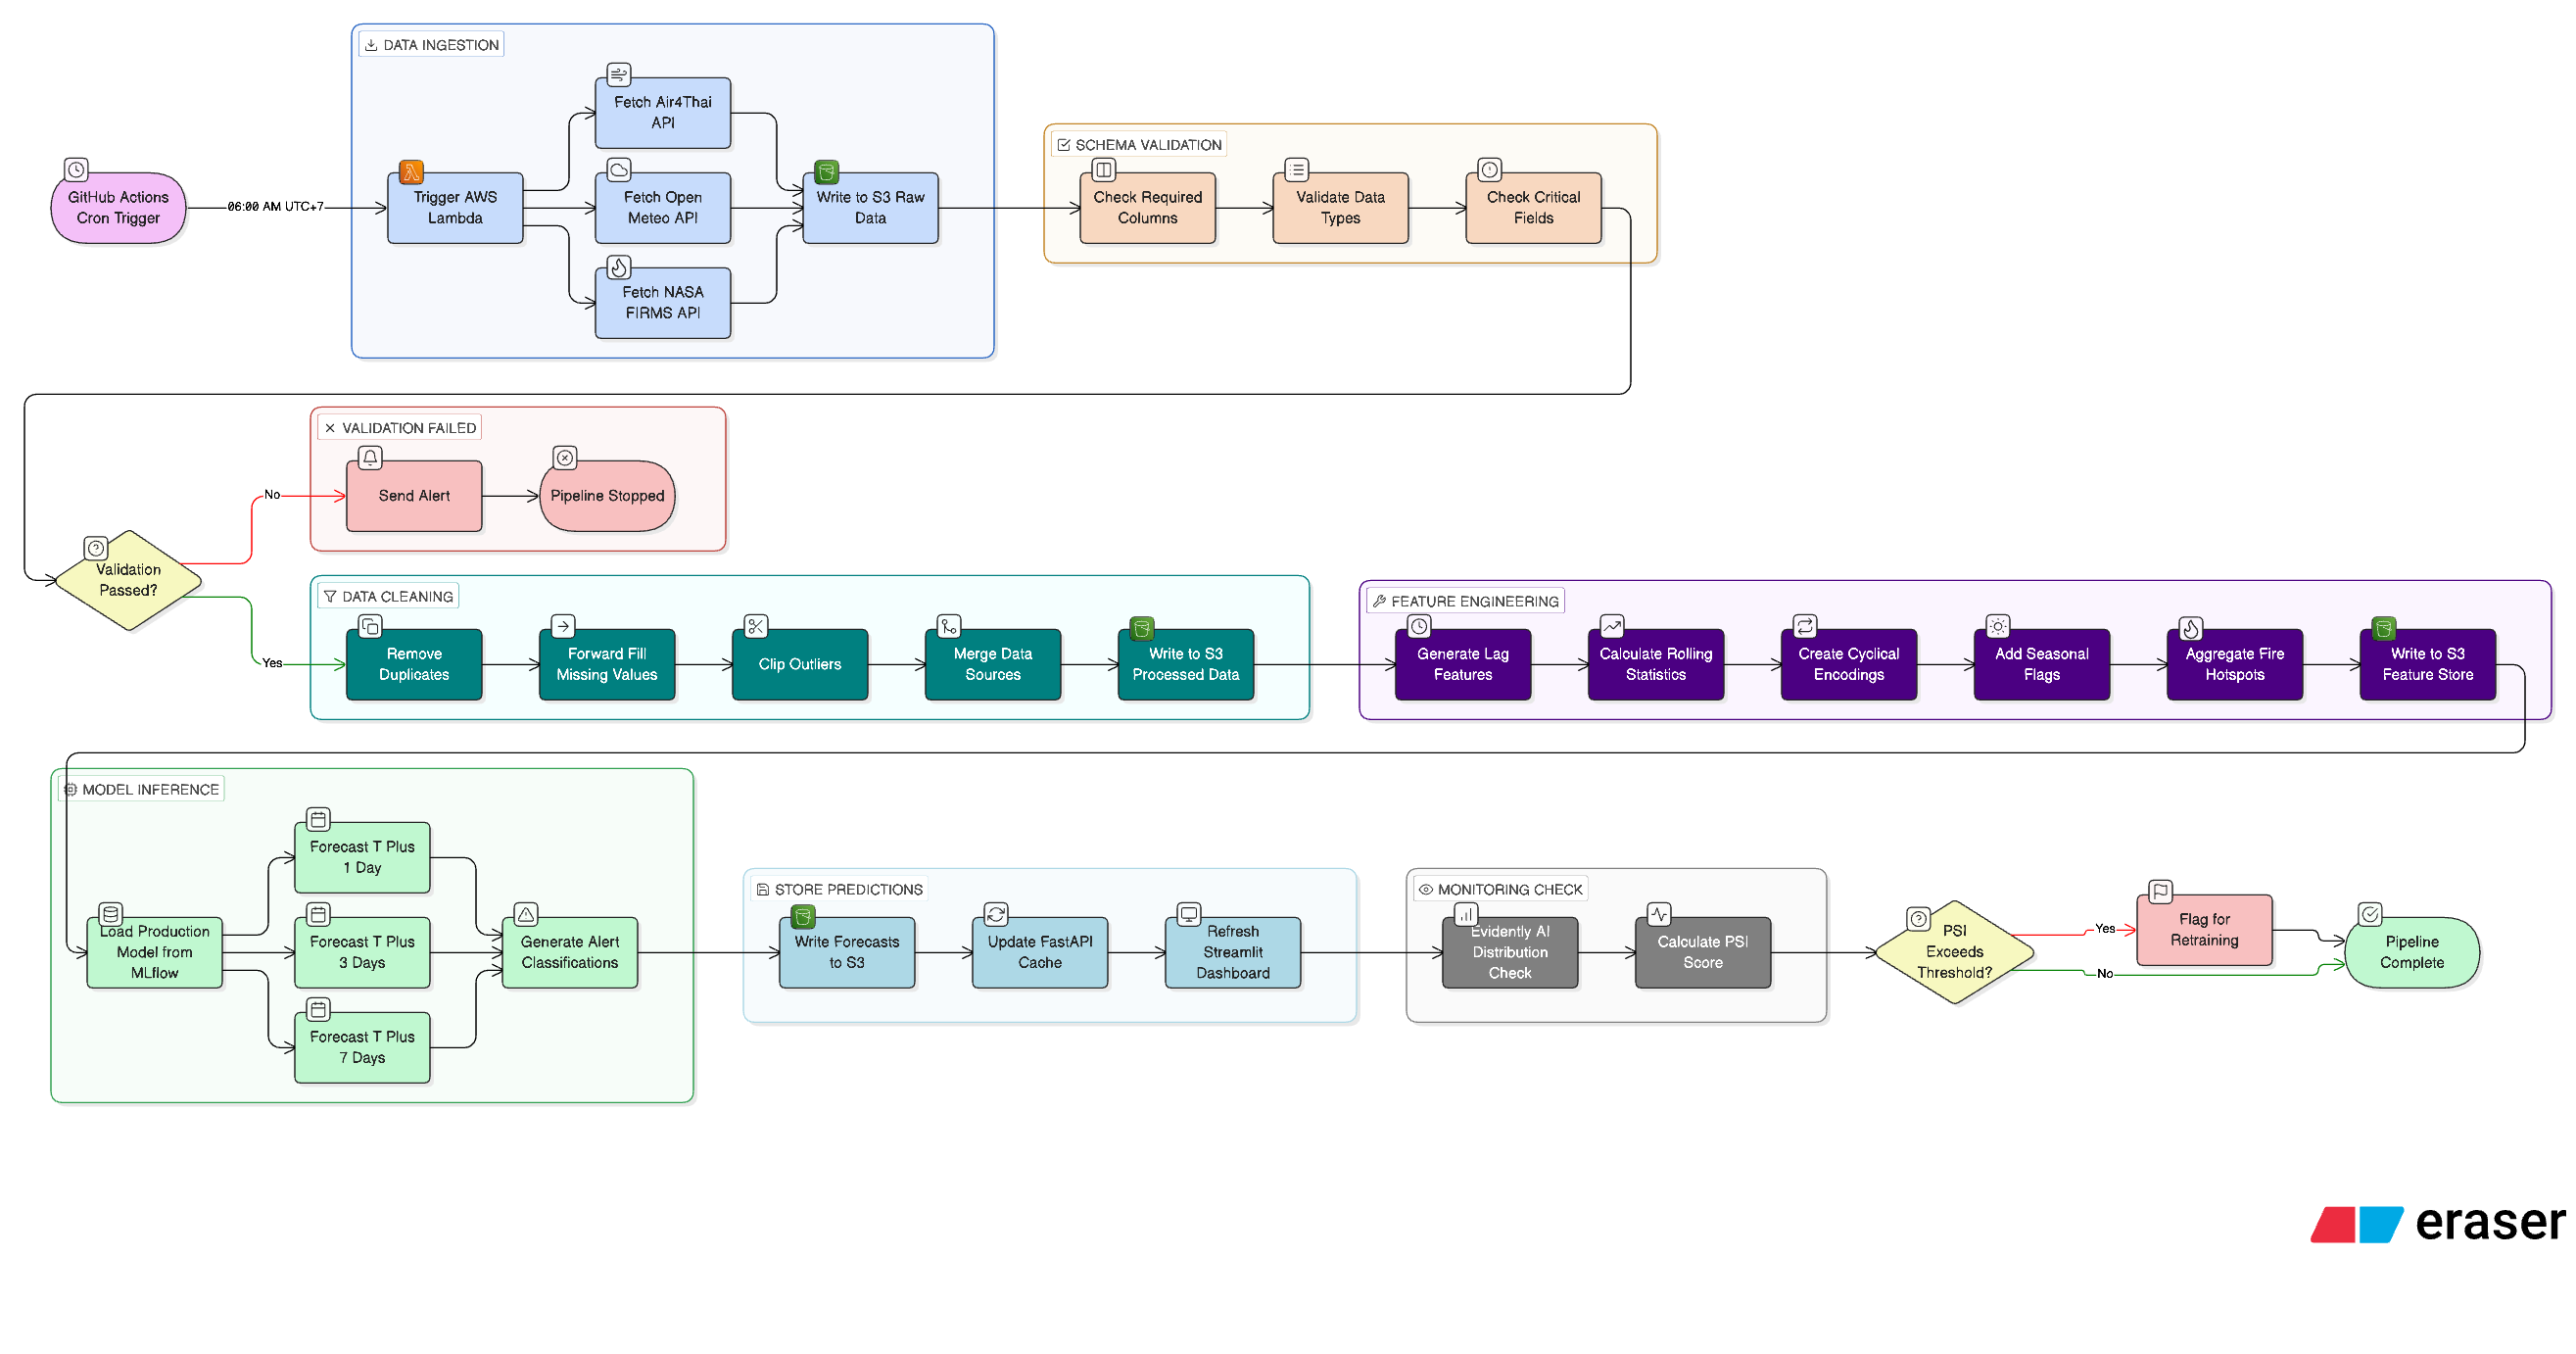
\includegraphics[width=0.85\textwidth]{fig_daily_pipeline}
    \caption{CAAS daily data pipeline — from ingestion to drift monitoring.}
    \label{fig:daily_pipeline}
\end{figure}

\section{Feature Engineering}

The feature matrix (\texttt{build\_features.py}) produces 45 features from the
three raw sources, grouped as follows:

\begin{table}[H]
\centering
\caption{CAAS Feature Groups}
\label{tab:features}
\begin{tabular}{llr}
\toprule
\textbf{Group} & \textbf{Features} & \textbf{Count} \\
\midrule
PM2.5 lags          & pm25\_lag1/3/7/14/30                                   & 5  \\
Rolling statistics  & roll3/7/14/30\_mean, roll7/14\_std                     & 6  \\
Temporal encodings  & month, week, day\_of\_year, sin/cos encodings, is\_haze\_season & 8  \\
Weather             & temp (max/min/mean), humidity (max/min), precipitation,
                      wind speed, wind direction (sin/cos), pressure,
                      cloud cover, evapotranspiration                        & 11 \\
Fire (FIRMS)        & hotspot\_50km, hotspot\_100km, mean\_frp\_50km,
                      hotspot\_7d\_roll, hotspot\_14d\_roll, fire\_flag      & 6  \\
Alert lags          & alert\_lag1/3/7                                         & 3  \\
Cross features      & lag1$\times$temp, lag1$\times$wind, roll7$\times$fire,
                      precip\_flag, humidity$\times$wind                     & 5  \\
\midrule
\textbf{Total}      &                                                         & \textbf{45} \\
\bottomrule
\end{tabular}
\end{table}

Key engineering decisions:
\begin{itemize}
    \item \textbf{No data leakage:} Lag and rolling features use only past values.
          Target columns (pm25\_t1, pm25\_t3, pm25\_t7) are forward-shifted.
    \item \textbf{Fire accumulation features:} 7-day and 14-day rolling hotspot
          counts capture the cumulative smoke load better than a single-day count.
    \item \textbf{Cyclic temporal encodings:} Month and day-of-year are encoded
          as sine/cosine pairs to preserve calendar continuity (December-January
          boundary).
    \item \textbf{Cross features:} lag1$\times$temp and roll7$\times$fire capture
          interactive effects between PM2.5 persistence and environmental conditions.
\end{itemize}

\section{Data Storage and Versioning}

All data artefacts are stored in Amazon S3 with a structured prefix layout:

\begin{verbatim}
s3://caas-mlops-bucket/
    data/raw/         ← original Excel and CSV files
    data/processed/   ← pm25_consolidated.csv, weather, FIRMS
    data/features/    ← features.csv (daily snapshot)
    models/           ← xgboost_t1/3/7.json (champion models)
    results/          ← forecasts, drift reports, summaries
    mlflow/           ← MLflow artefacts
\end{verbatim}

S3 bucket versioning is enabled, preserving every version of model files
and allowing rollback to any previous champion.

\section{Pipeline Orchestration}

Pipeline scheduling is handled by GitHub Actions:
\begin{itemize}
    \item \textbf{daily\_pipeline.yml} --- cron 06:00 Bangkok time, runs ingest +
          inference + upload + drift check.
    \item \textbf{retrain.yml} --- triggered annually (December~1) or on-demand
          via \texttt{repository\_dispatch} from the drift monitor.
    \item \textbf{test.yml} --- runs pytest suite on every push to main.
\end{itemize}

This architecture was chosen over Apache Airflow for simplicity within the
capstone scope. Airflow would be appropriate for multi-team production use
requiring finer DAG-level observability and retries.

\chapter{Machine Learning Model Development}
\label{ch:ml-development}

\section{Dataset and Splits}

The feature matrix contains 5,257 daily records spanning May~2011 to
December~2025. A strict chronological split was applied to prevent data leakage:

\begin{table}[H]
\centering
\caption{Train / Validation / Test Split}
\begin{tabular}{llr}
\toprule
\textbf{Split} & \textbf{Period} & \textbf{Rows} \\
\midrule
Train      & 2011-05-18 → 2022-12-31 & 4,160 \\
Validation & 2023-01-01 → 2023-12-31 &   365 \\
Test       & 2024-01-01 → 2025-12-31 &   731 \\
\bottomrule
\end{tabular}
\end{table}

All preprocessing (median imputation, scaling) was fitted exclusively on the
training set and applied to validation and test sets without look-ahead.

\section{Baseline}

A persistence baseline was established using yesterday's PM2.5 value as the
forecast for all horizons. This represents the simplest possible model and
provides a floor that any learned model must surpass.

\begin{table}[H]
\centering
\caption{Persistence Baseline — Test MAE}
\begin{tabular}{lr}
\toprule
\textbf{Horizon} & \textbf{MAE (µg/m³)} \\
\midrule
t+1 & 5.30 \\
t+3 & 8.97 \\
t+7 & 10.93 \\
\bottomrule
\end{tabular}
\end{table}

\section{Model Selection}

Three model families were evaluated under an Optuna-driven hyperparameter search
(100+ trials per family per horizon), all sharing the same 45-feature input and
chronological split:

\textbf{LightGBM} was selected as the \emph{champion}. It combines the
efficiency of histogram-based boosting with strong tabular performance and sub-5ms
inference per row, and outperformed both competitors on every horizon. Best
hyperparameters at t+1 include 357 estimators, 255 leaves, max\_depth=6,
learning\_rate $\approx$ 0.043; longer horizons use deeper, more regularised
configurations.

\textbf{XGBoost} was retained as a \emph{strong secondary} and runtime fallback:
it is architecturally close to the LightGBM champion, trails it by $<$~0.3~MAE
at every horizon, and is exposed on the FastAPI service as
\texttt{?model=xgboost} for A/B comparison.

\textbf{LSTM} was trained as a \emph{comparison baseline} to assess whether
temporal sequence structure adds value over tabular lag features. The tuned
architecture (Optuna search over arch~$\in$~\{LSTM, Attention, CNN-LSTM\},
seq\_len, hidden units, dropout, learning rate) converges to architecture-horizon
pairs (attention @ seq=7 for t+1, CNN-LSTM @ seq=30 for t+3).

\section{Results}

\subsection{LightGBM (Champion)}

\begin{table}[H]
\centering
\caption{LightGBM Test Set Performance}
\label{tab:lgbm_results}
\begin{tabular}{lrrrr}
\toprule
\textbf{Horizon} & \textbf{MAE} & \textbf{RMSE} & \textbf{R²} & \textbf{AUROC} \\
\midrule
t+1 & 5.12 & 9.00  & 0.841 & 0.992 \\
t+3 & 6.77 & 11.78 & 0.729 & 0.973 \\
t+7 & 8.25 & 14.36 & 0.600 & 0.946 \\
\bottomrule
\end{tabular}
\end{table}

LightGBM beats the persistence baseline at every horizon: MAE improvement is
+3\% at t+1, +25\% at t+3, and +25\% at t+7. The +3\% lift at t+1 is modest
because same-day PM2.5 is an extremely strong anchor (the lag-1 signal), and
any learned model must push past that ceiling using fire + weather features.

\subsection{XGBoost (Strong Secondary)}

\begin{table}[H]
\centering
\caption{XGBoost Test Set Performance (Optuna-tuned)}
\label{tab:xgb_results}
\begin{tabular}{lrrrr}
\toprule
\textbf{Horizon} & \textbf{MAE} & \textbf{RMSE} & \textbf{R²} & \textbf{AUROC} \\
\midrule
t+1 & 5.31 & 8.95  & 0.843 & 0.992 \\
t+3 & 7.08 & 11.90 & 0.723 & 0.973 \\
t+7 & 8.90 & 15.32 & 0.544 & 0.933 \\
\bottomrule
\end{tabular}
\end{table}

XGBoost trails the LightGBM champion by 0.19--0.65~MAE across horizons. The gap
widens at t+7, where LightGBM's histogram-based leaf growth generalises slightly
better on the harder long-range task. XGBoost is kept loaded in the FastAPI
service as a runtime fallback (\texttt{?model=xgboost}) and as an independent
score for threshold-based A/B comparison.

\subsection{LSTM (Comparison)}

\begin{table}[H]
\centering
\caption{LSTM Test Set Performance}
\label{tab:lstm_results}
\begin{tabular}{lrrr}
\toprule
\textbf{Horizon} & \textbf{MAE} & \textbf{RMSE} & \textbf{R²} \\
\midrule
t+1 & 6.67 & 11.64 & 0.753 \\
t+3 & 8.87 & 15.89 & 0.540 \\
t+7 & 8.06 & 14.49 & 0.608 \\
\bottomrule
\end{tabular}
\end{table}

Both gradient-boosted models outperform LSTM at t+1 (MAE 5.12 / 5.31 vs.\ 6.67)
and t+3 (6.77 / 7.08 vs.\ 8.87), while performance at t+7 is comparable
(8.25 / 8.90 vs.\ 8.06). The LSTM's weaker t+3 result (R²=0.54) reflects the
difficulty of the mid-range horizon, where the recency of lag features decays
but seasonal signals are not yet dominant. LightGBM is selected as the champion.

\subsection{Actual vs.\ Predicted}

\begin{figure}[H]
    \centering
    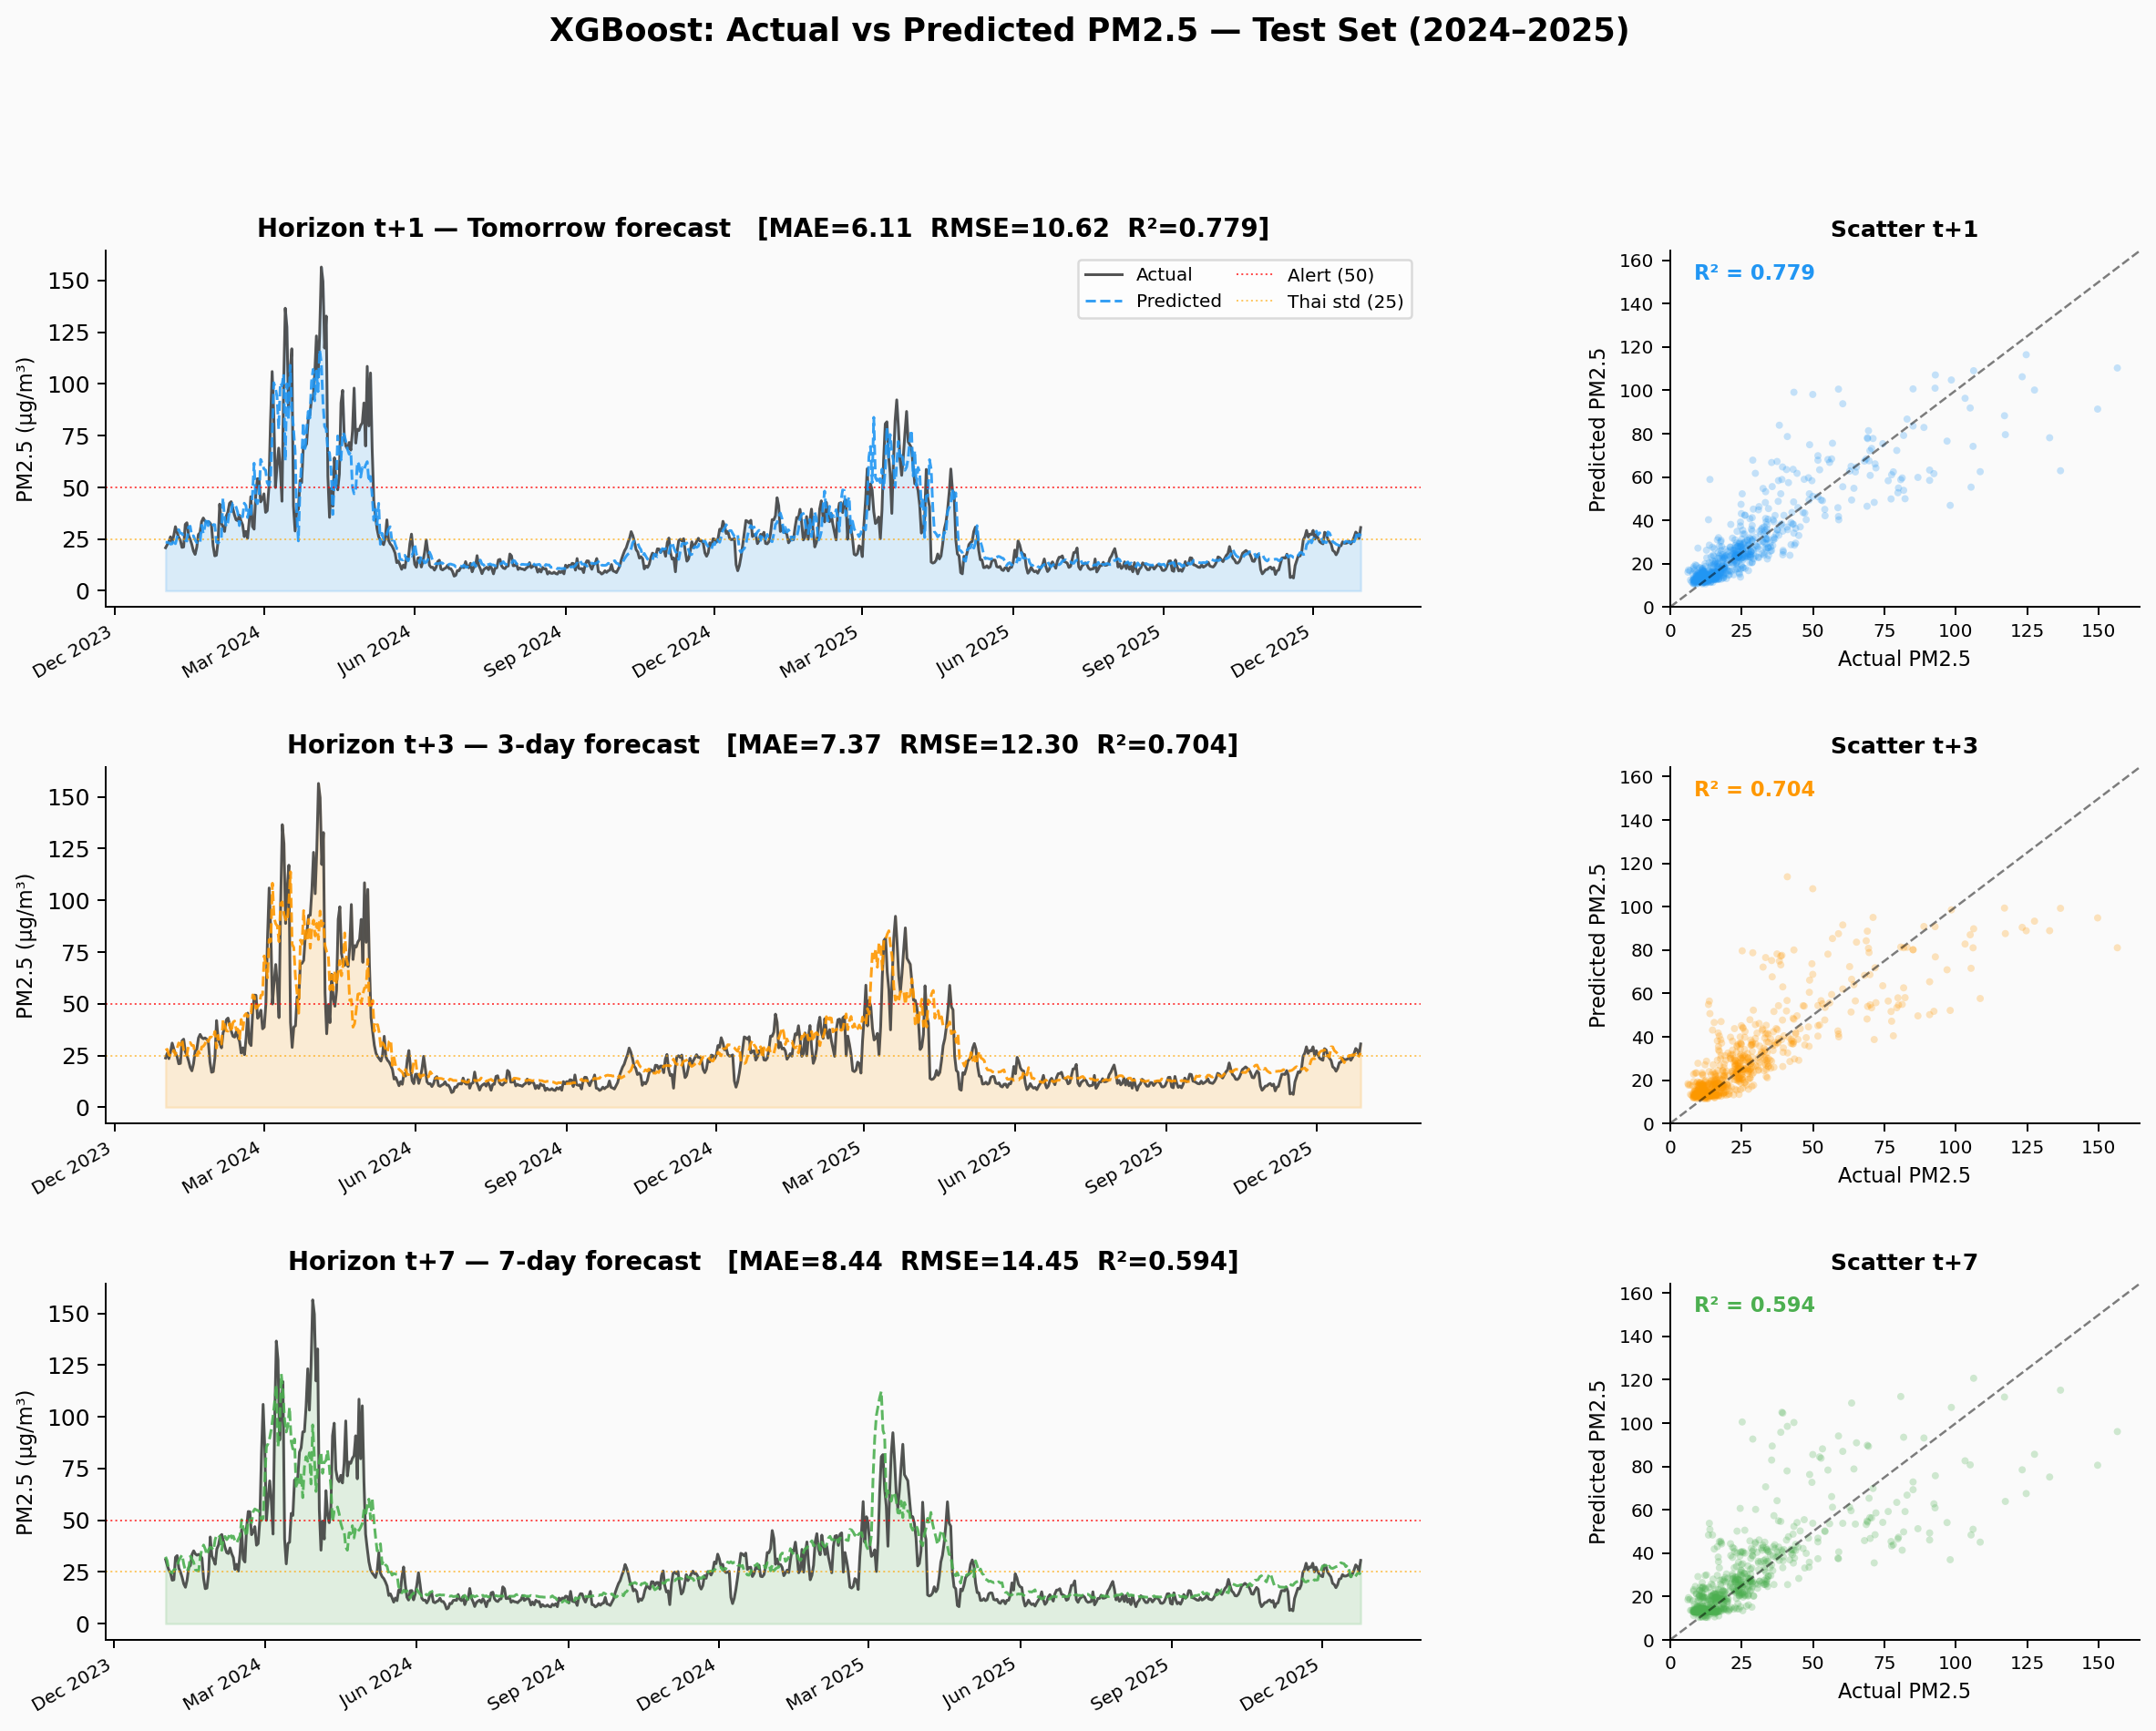
\includegraphics[width=0.9\textwidth]{fig_actual_vs_predicted}
    \caption{Champion t+1 actual vs.\ predicted PM2.5 on the 2024--2025 test set.
             The model captures seasonal haze peaks accurately.}
    \label{fig:actual_vs_predicted}
\end{figure}

\section{Ablation Study: FIRMS Fire Data}

To quantify the contribution of NASA FIRMS fire hotspot features, Scenario~D
retrained the XGBoost candidate with the six FIRMS-derived features removed
(39 features total) and compared against the full-feature XGBoost run from the
same training harness. Using XGBoost rather than the LightGBM champion isolates
the ablation from concurrent hyperparameter differences.

\begin{table}[H]
\centering
\caption{Scenario D — MAE Impact of Removing FIRMS Features (XGBoost)}
\begin{tabular}{lrrr}
\toprule
\textbf{Horizon} & \textbf{Full MAE} & \textbf{No-FIRMS MAE} & \textbf{MAE increase} \\
\midrule
t+1 & 6.11 & 6.52 & +6.8\% \\
t+3 & 7.37 & 7.75 & +5.1\% \\
t+7 & 8.44 & 8.80 & +4.3\% \\
\bottomrule
\end{tabular}
\end{table}

Fire data provides consistent, measurable improvement across all horizons.
The effect is strongest at t+1 (6.8\%), where recent hotspot counts directly
predict tomorrow's PM2.5 accumulation.

\begin{figure}[H]
    \centering
    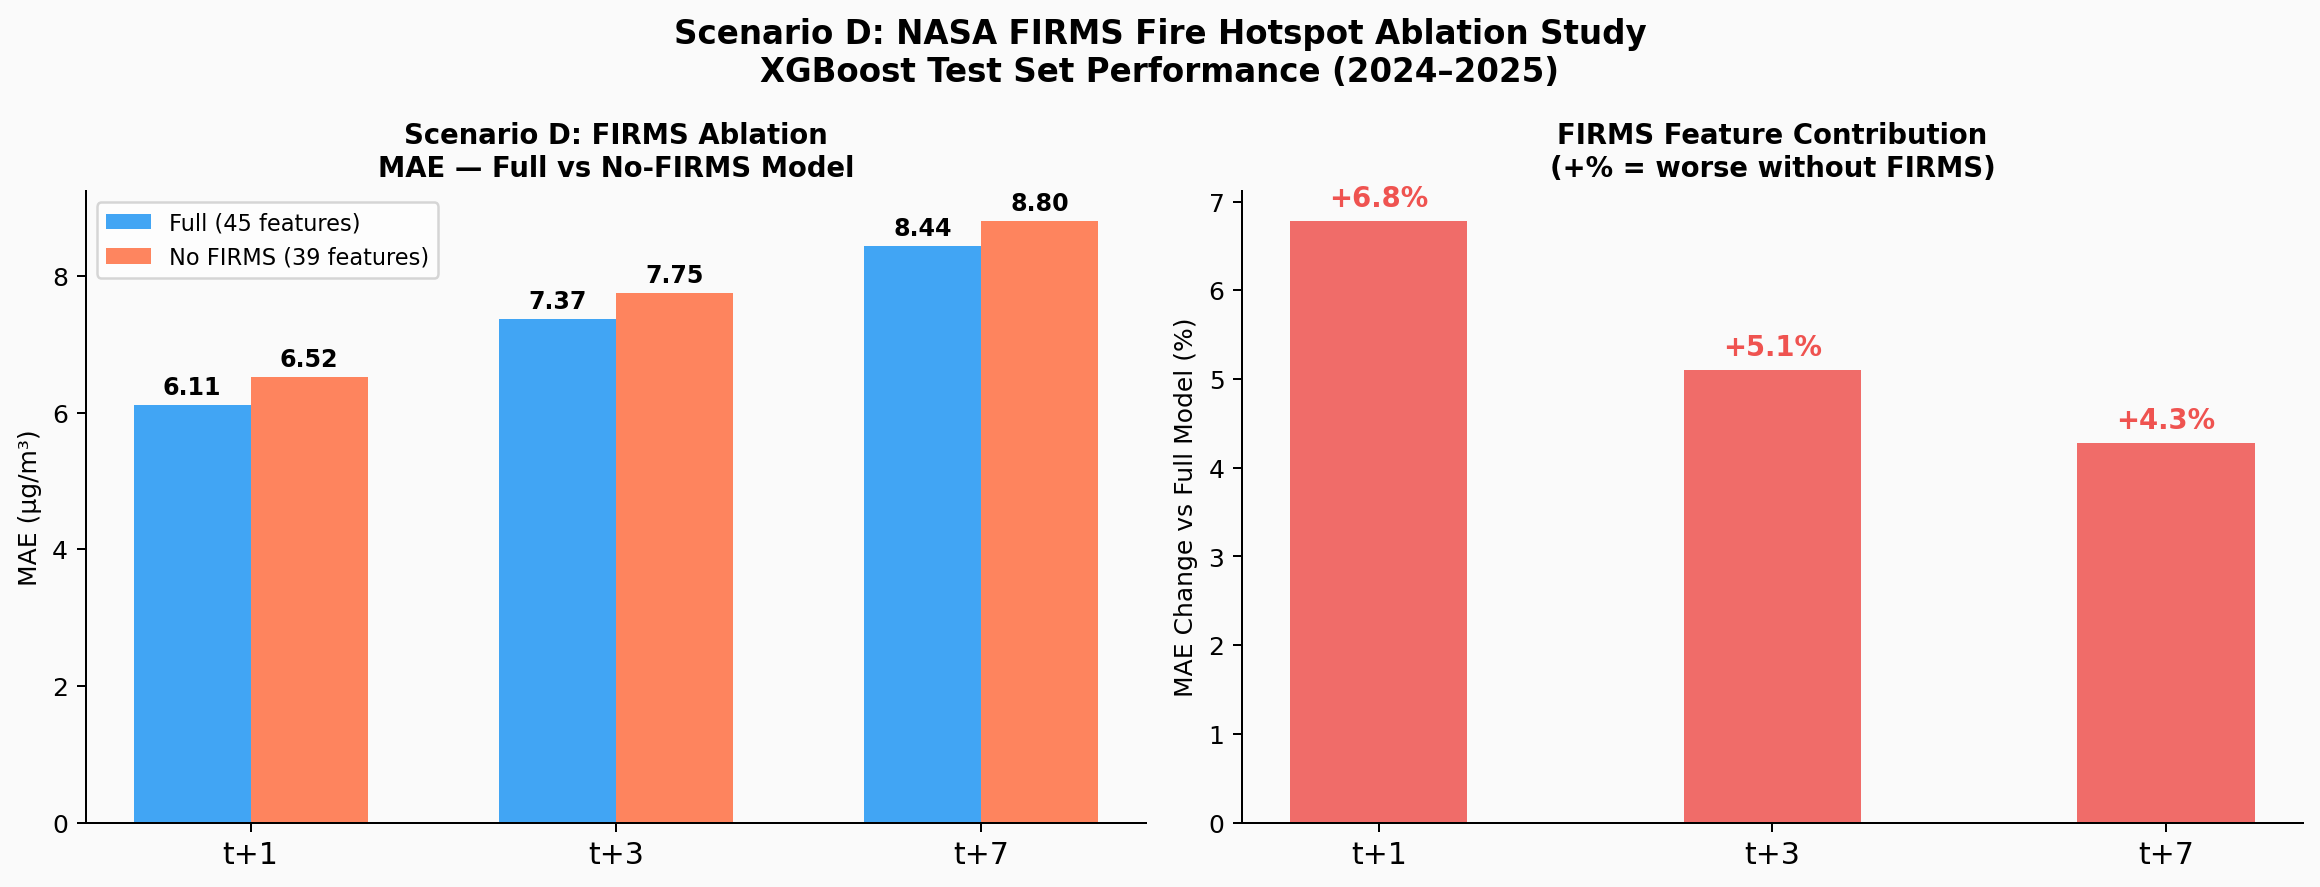
\includegraphics[width=0.75\textwidth]{fig_firms_ablation}
    \caption{MAE comparison: full model vs.\ model without FIRMS fire features.}
    \label{fig:firms_ablation}
\end{figure}

\section{Alert Classifier Analysis (Scenario C)}

The binary hazard alert (PM2.5 $>$ 50~\textmu g/m\textsuperscript{3}) is derived
from the regression output by applying a threshold. Scenario~C investigated
whether the default 50~\textmu g/m\textsuperscript{3} threshold is optimal by
computing F1 score across all possible thresholds on the test set.

\begin{table}[H]
\centering
\caption{Scenario C — Alert Threshold Optimisation (XGBoost scores)}
\begin{tabular}{lrrrr}
\toprule
\textbf{Horizon} & \textbf{Default (50)} & \textbf{Optimal threshold} & \textbf{Default F1} & \textbf{Optimal F1} \\
\midrule
t+1 & 50.0 µg/m³ & 53.7 µg/m³ & 0.839 & \textbf{0.879} \\
t+3 & 50.0 µg/m³ & 51.0 µg/m³ & 0.787 & \textbf{0.789} \\
t+7 & 50.0 µg/m³ & 45.8 µg/m³ & 0.684 & \textbf{0.695} \\
\bottomrule
\end{tabular}
\end{table}

Threshold tuning was performed against the XGBoost test-set predictions (the
regression scores the same pipeline exposes as \texttt{?model=xgboost}) so that
each alert class is evaluated on an unbiased held-out split. The standard
50~\textmu g/m\textsuperscript{3} threshold is near-optimal for t+3 and t+7.
For t+1, raising the threshold to 53.7~\textmu g/m\textsuperscript{3} reduces
false alarms (precision 0.769 → 0.885) while maintaining recall
(0.924 → 0.873), yielding a +4.0\% F1 gain.

\begin{figure}[H]
    \centering
    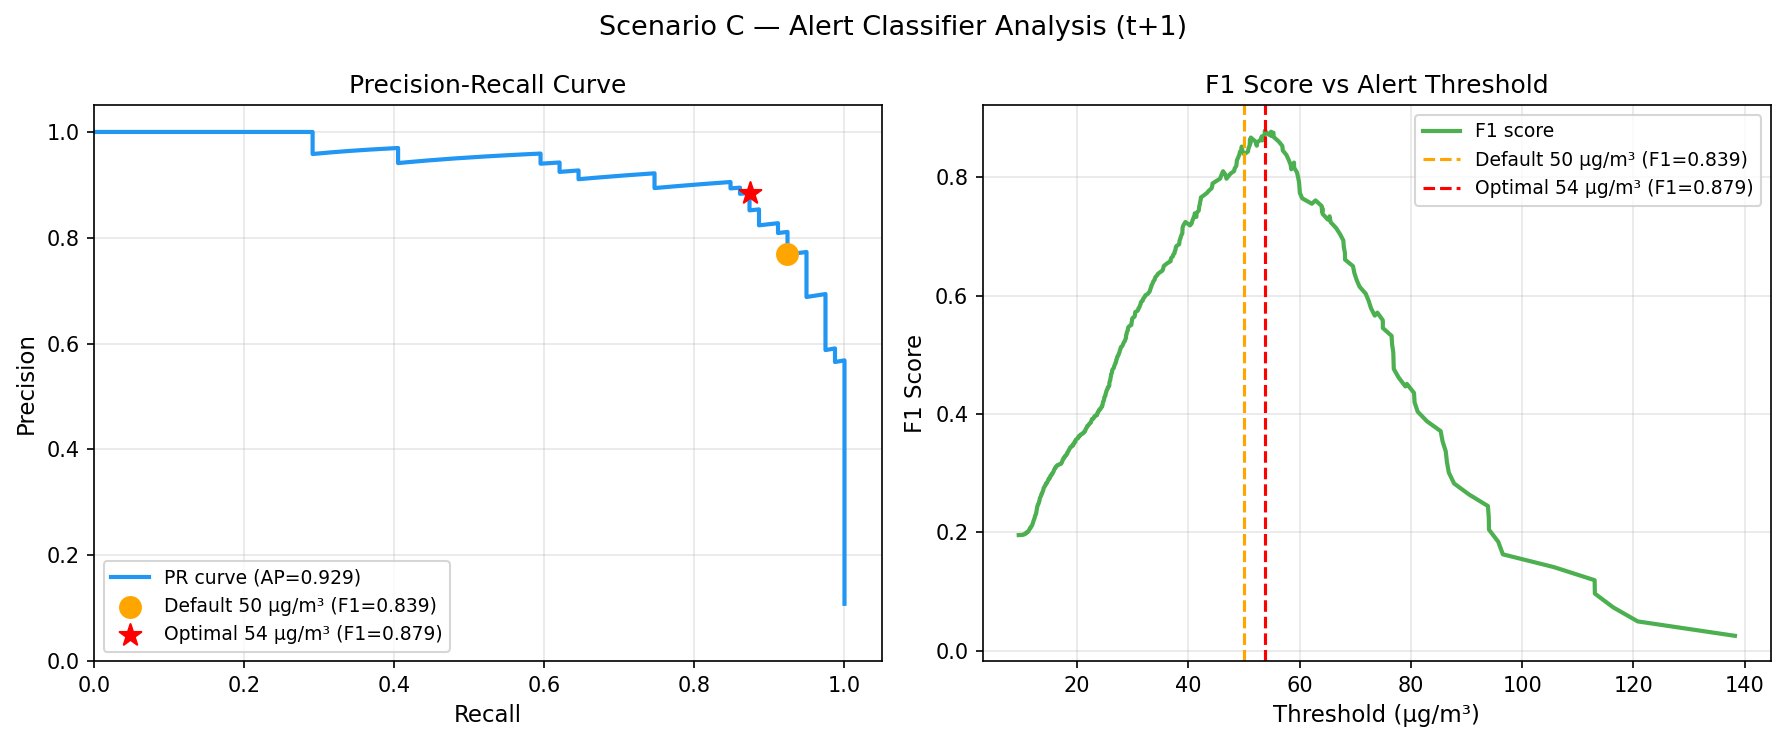
\includegraphics[width=\textwidth]{fig_pr_curve_t1}
    \caption{Precision-recall curve and F1 vs.\ threshold for t+1 alert classifier.}
    \label{fig:pr_curve_t1}
\end{figure}

\section{Model Interpretation (SHAP)}

SHAP (SHapley Additive exPlanations) values were computed against the XGBoost
strong-secondary on the test set. XGBoost shares LightGBM's underlying gradient-
boosted tree structure and exposes the same 45-feature input, so its SHAP
attributions are representative of the broader gradient-boosting regime; running
SHAP on XGBoost avoids LightGBM's TreeExplainer compatibility caveats while
preserving the physical interpretation story.

\begin{figure}[H]
    \centering
    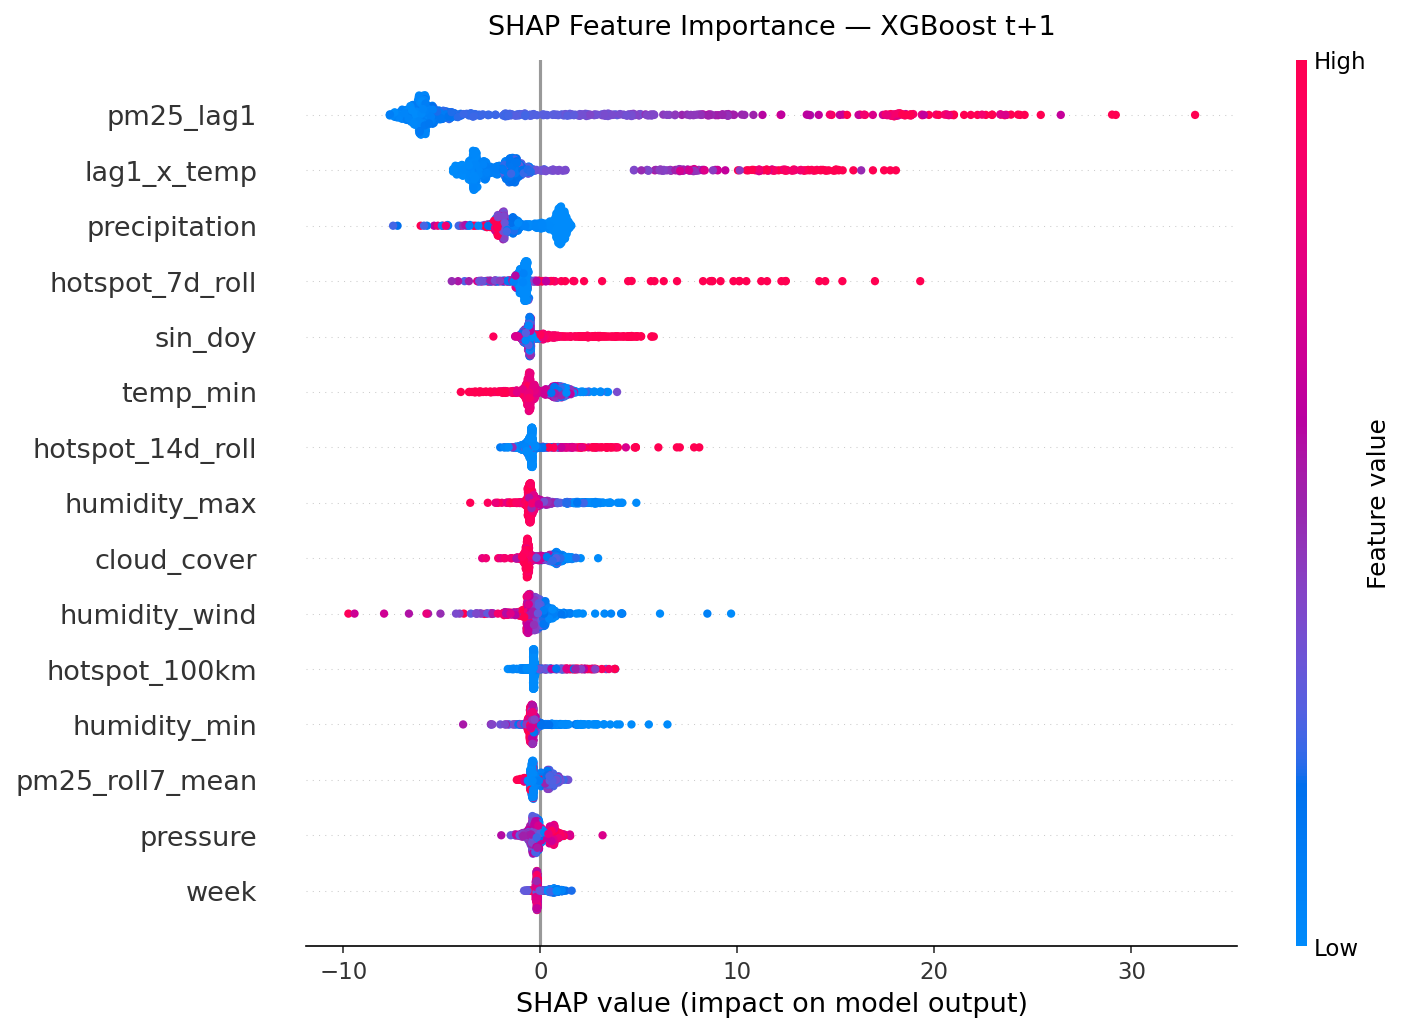
\includegraphics[width=0.85\textwidth]{fig_shap_summary_t1}
    \caption{SHAP summary plot at t+1. \texttt{pm25\_lag1} dominates,
    confirming that next-day PM2.5 is primarily driven by today's concentration.}
    \label{fig:shap_t1}
\end{figure}

\begin{figure}[H]
    \centering
    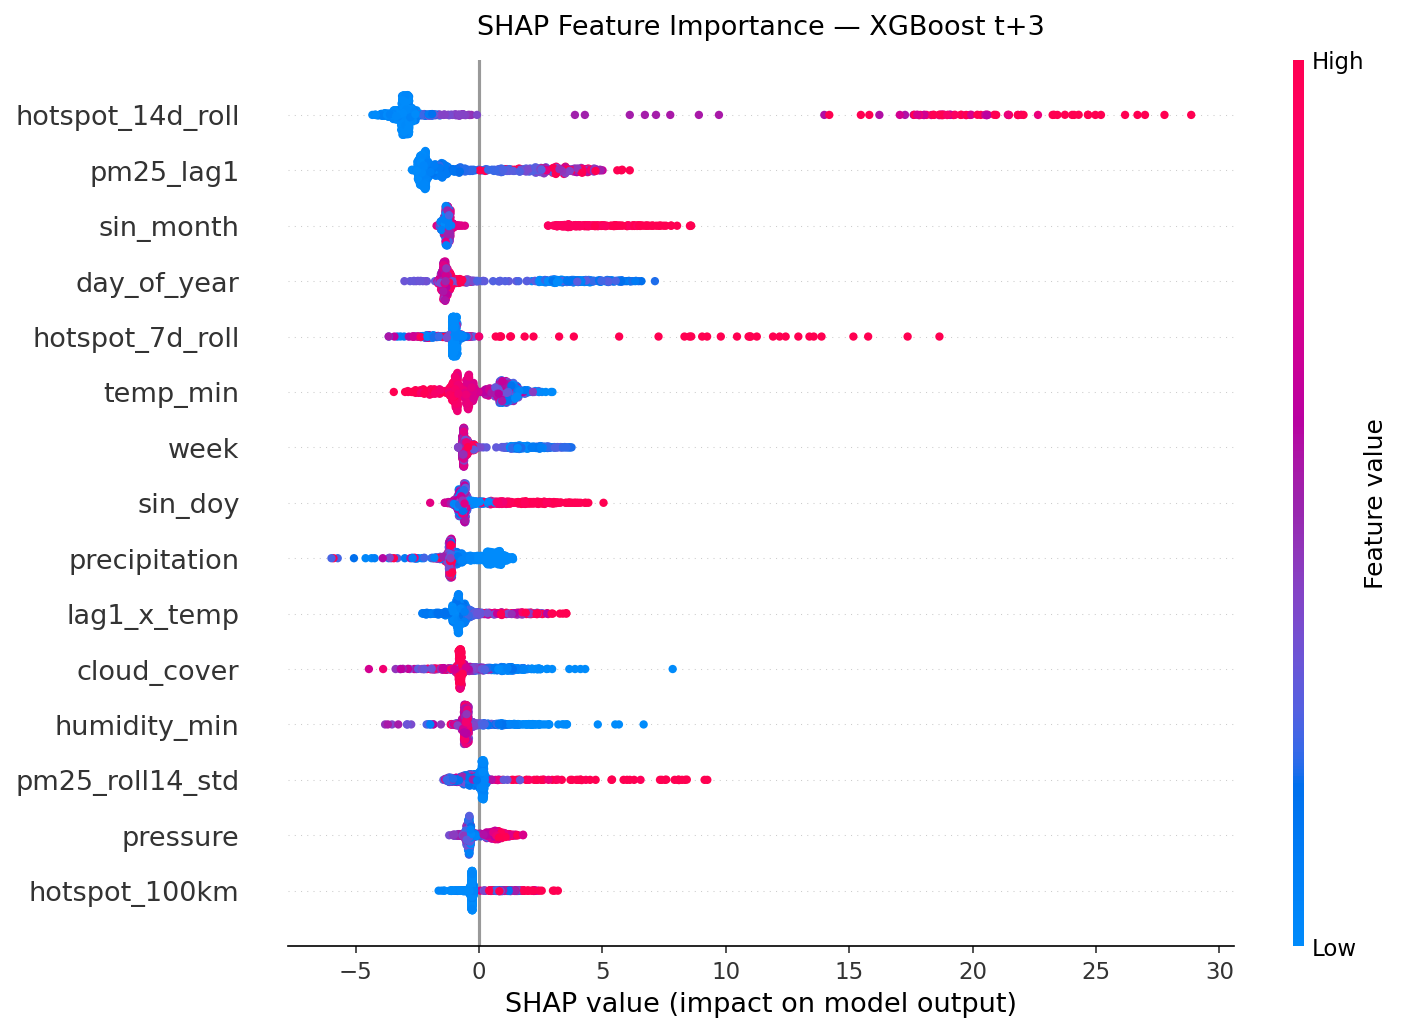
\includegraphics[width=0.85\textwidth]{fig_shap_summary_t3}
    \caption{SHAP summary plot at t+3. \texttt{hotspot\_14d\_roll} becomes
    the dominant signal, reflecting fire accumulation over two weeks.}
    \label{fig:shap_t3}
\end{figure}

A key insight is that the dominant predictive signal shifts with horizon:
\begin{itemize}
    \item \textbf{t+1:} Recent PM2.5 (\texttt{pm25\_lag1}, mean SHAP = 6.85) ---
          next-day concentration is primarily a persistence phenomenon.
    \item \textbf{t+3:} 14-day fire accumulation (\texttt{hotspot\_14d\_roll}, 4.63)
          --- two-week fire buildup is the strongest medium-range signal.
    \item \textbf{t+7:} Seasonal position (\texttt{sin\_month}, 4.63;
          \texttt{hotspot\_7d\_roll}, 3.00) --- at 7 days, the model relies on
          calendar position within the haze season plus near-term fire activity.
\end{itemize}

This gradient from measurement-driven to climatology-driven prediction is
consistent with the physical understanding of PM2.5 dynamics in Chiang Mai.

\chapter{MLOps Implementation}
\label{ch:mlops}

\section{System Architecture}

Figure~\ref{fig:architecture} shows the end-to-end CAAS architecture.
Data flows from three external sources through an automated ingestion pipeline
into a feature store (Amazon S3), is used to train and register models in
MLflow, served via FastAPI on EC2, and monitored continuously by Evidently.

\begin{figure}[H]
    \centering
    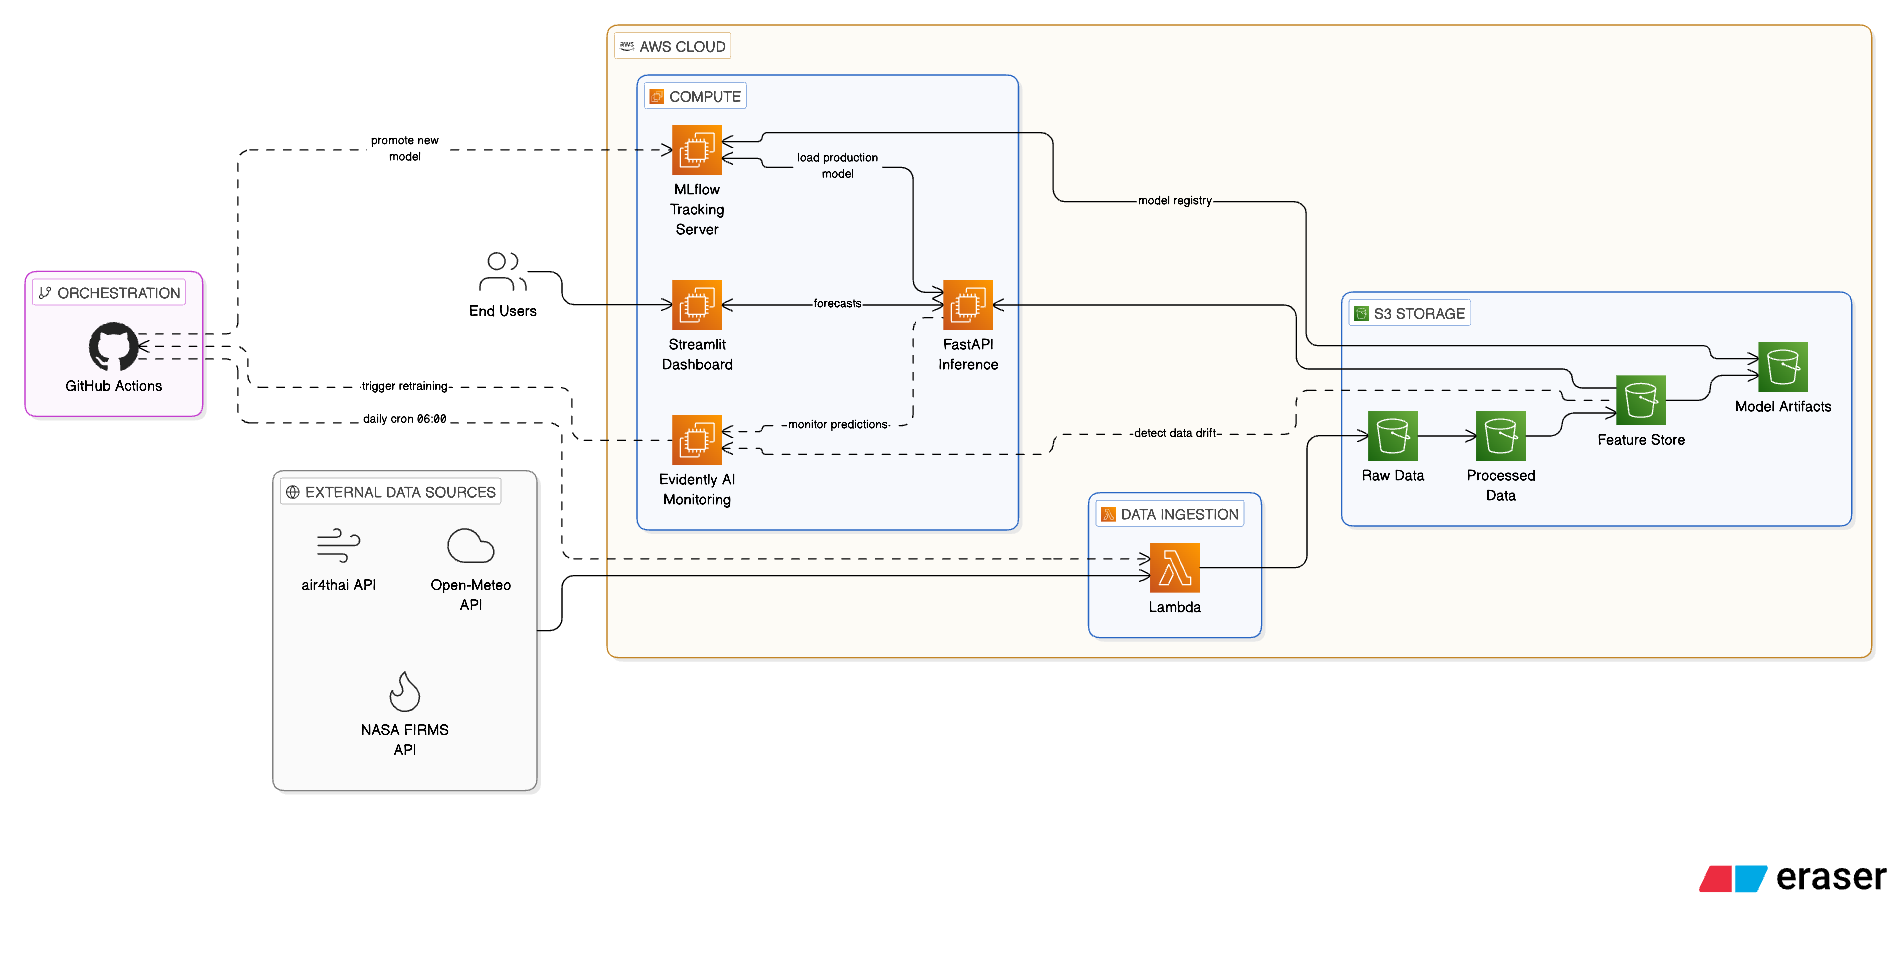
\includegraphics[width=\textwidth]{fig_cloud_architecture}
    \caption{CAAS cloud architecture on AWS. Three external APIs (air4thai,
    Open-Meteo, NASA FIRMS) feed a GitHub Actions-orchestrated ingestion layer
    (3-hourly cron) into four S3 tiers (Raw, Processed, Feature Store, Model
    Artifacts). A single EC2~t3.micro instance hosts FastAPI, MLflow, and
    Streamlit. Evidently AI drift monitoring runs as a daily scheduled job.}
    \label{fig:architecture}
\end{figure}

\section{Experiment Tracking and Model Registry}

All training runs are logged to MLflow with:
\begin{itemize}
    \item Full hyperparameter sets per horizon.
    \item Validation and test metrics (MAE, RMSE, R², alert F1, AUROC).
    \item Model artefacts (\texttt{.json} for XGBoost, \texttt{.keras} for LSTM).
    \item Feature importance and prediction CSVs as run artefacts.
\end{itemize}

Three experiments are maintained: \texttt{CAAS-XGBoost} (3 runs),
\texttt{CAAS-LSTM} (3 runs), and \texttt{CAAS-Ablation-NoFIRMS} (3 runs).

\begin{figure}[H]
    \centering
    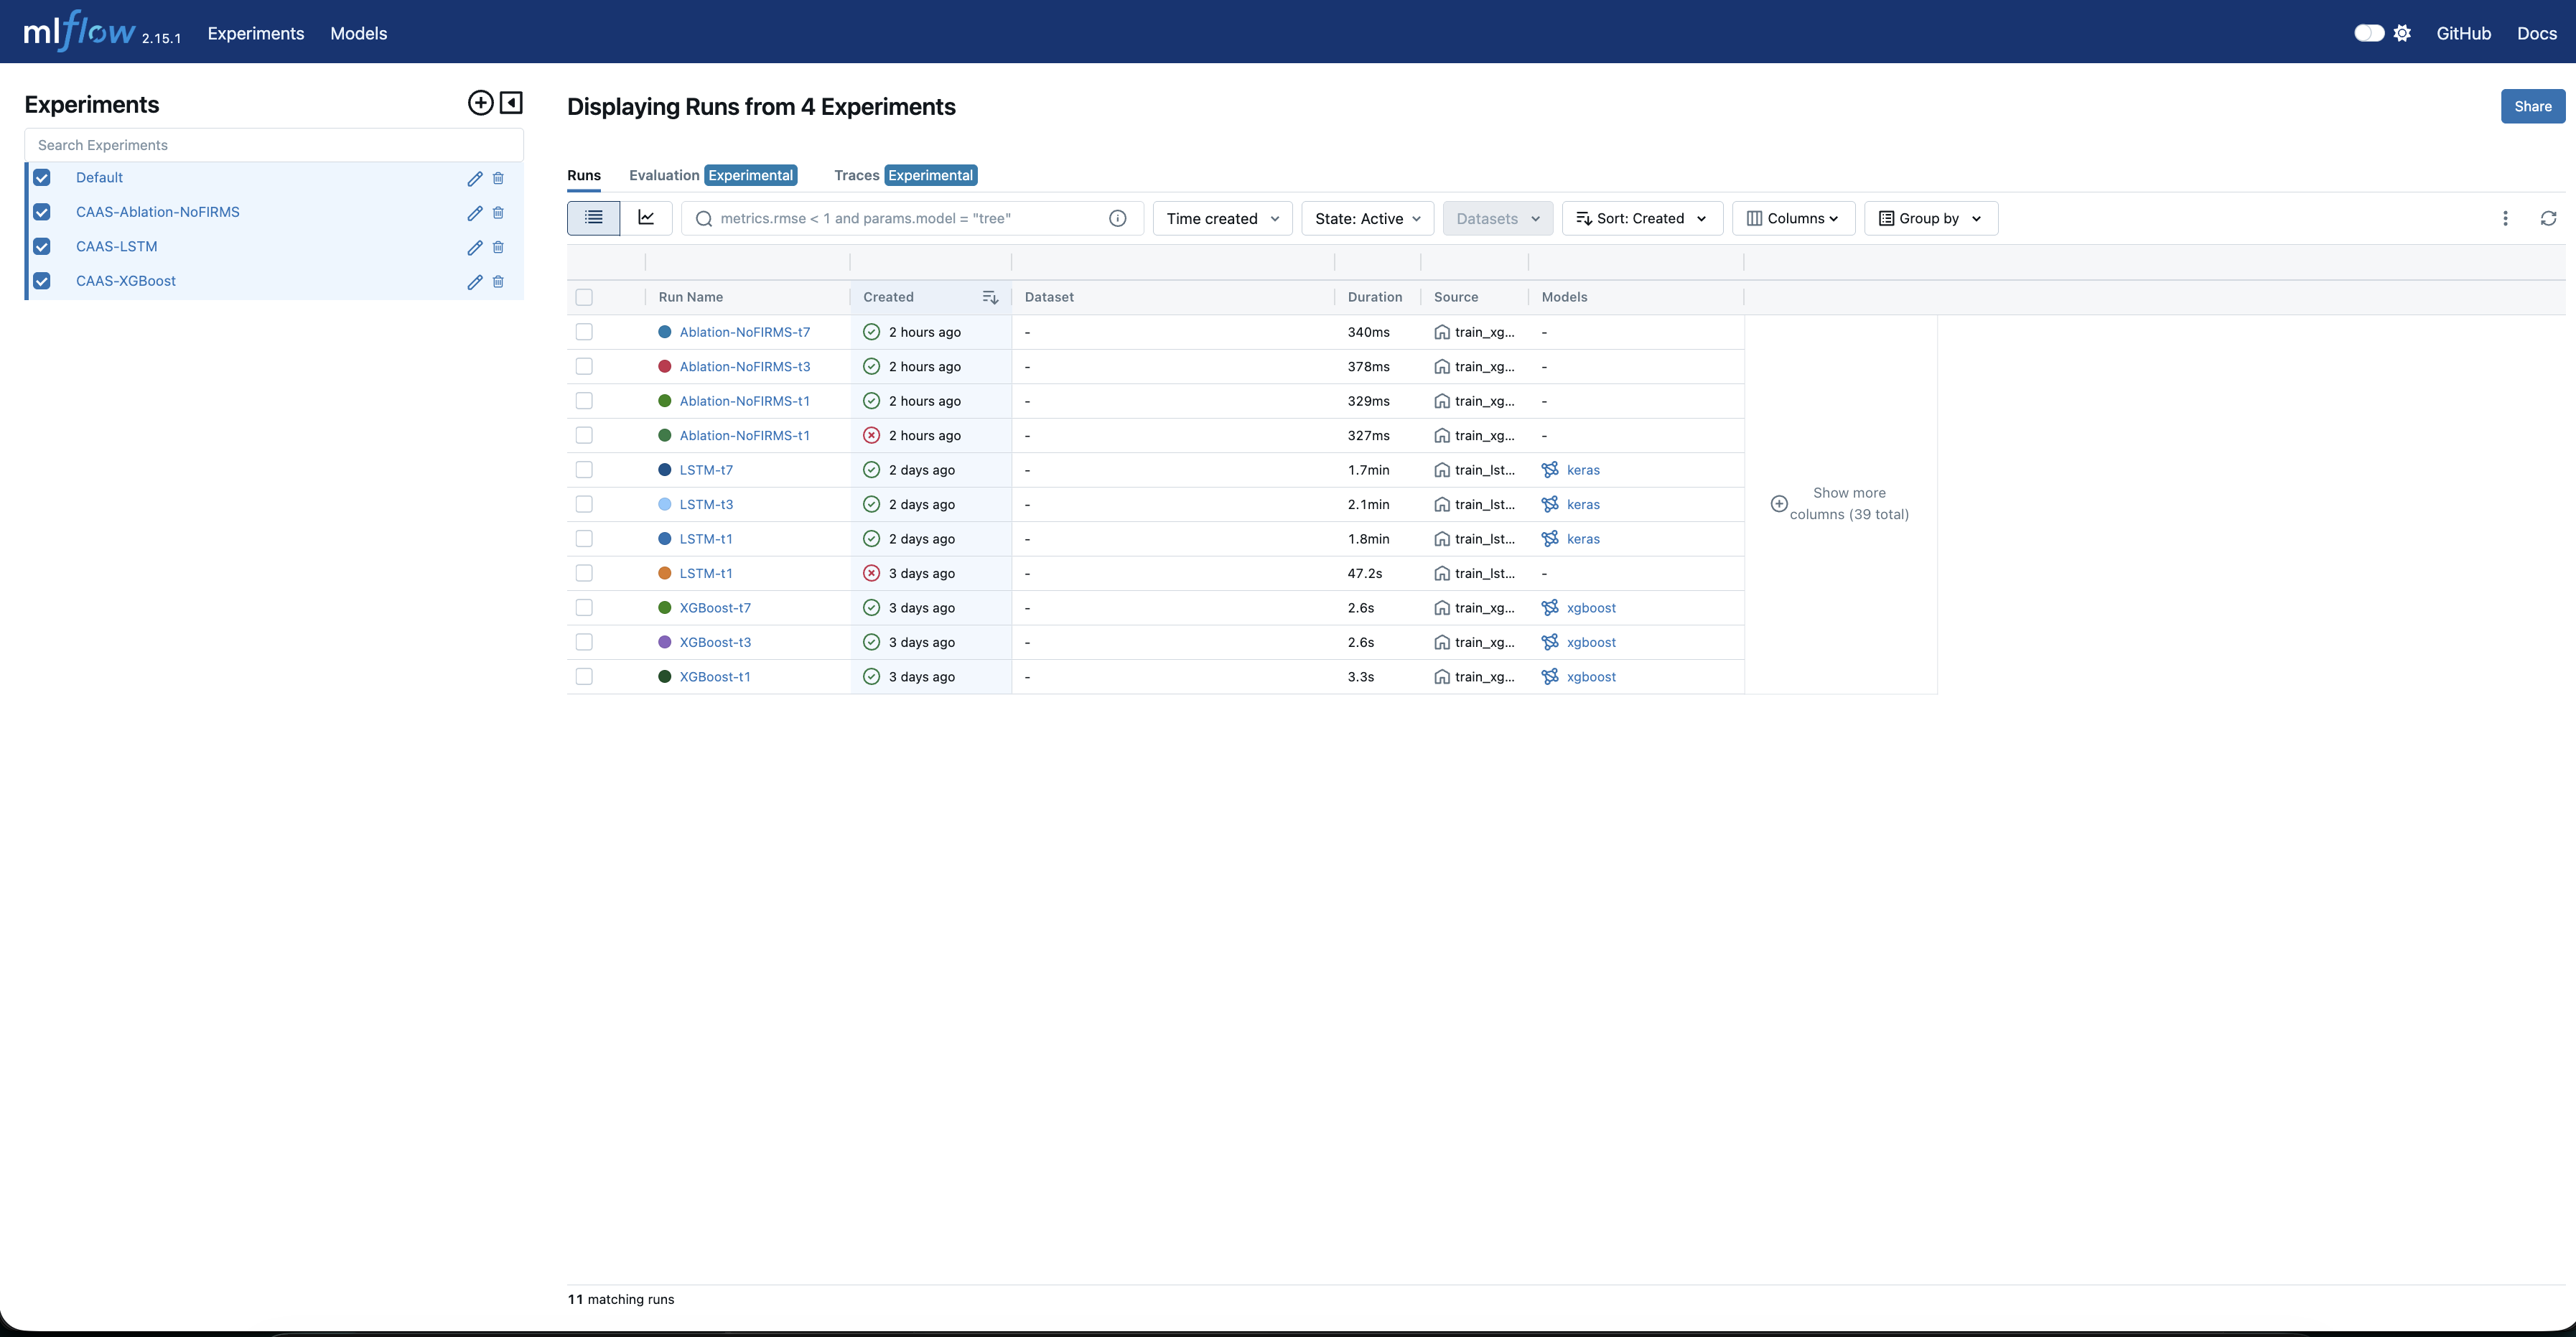
\includegraphics[width=0.85\textwidth]{fig_mlflow_runs}
    \caption{MLflow experiment view showing CAAS-XGBoost runs.}
    \label{fig:mlflow_runs}
\end{figure}

\section{Model Serving}

The champion XGBoost model is served via a FastAPI application
(\texttt{04\_Scripts/serve/app.py}) exposing five endpoints:

\begin{table}[H]
\centering
\caption{CAAS API Endpoints}
\begin{tabular}{llp{7cm}}
\toprule
\textbf{Method} & \textbf{Endpoint} & \textbf{Description} \\
\midrule
GET  & \texttt{/health}      & Liveness check, lists loaded models \\
GET  & \texttt{/forecast}    & Latest t+1/3/7 forecasts from most recent feature row \\
POST & \texttt{/predict}     & On-demand prediction from supplied feature values \\
GET  & \texttt{/history}     & Recent PM2.5 history for dashboard charting \\
GET  & \texttt{/model/info}  & Champion model metadata and test metrics \\
\bottomrule
\end{tabular}
\end{table}

The service is containerised using a multi-stage Docker build that reduces
the image size to approximately 300~MB by excluding training and monitoring
dependencies. On EC2, the container starts automatically via a user-data
bootstrap script that pulls the latest model artefacts from S3 at launch.

A Streamlit dashboard (\texttt{dashboard.py}) provides a public-facing
interface showing colour-coded forecast cards, a 60-day PM2.5 history chart,
and the model performance summary.

\begin{figure}[H]
    \centering
    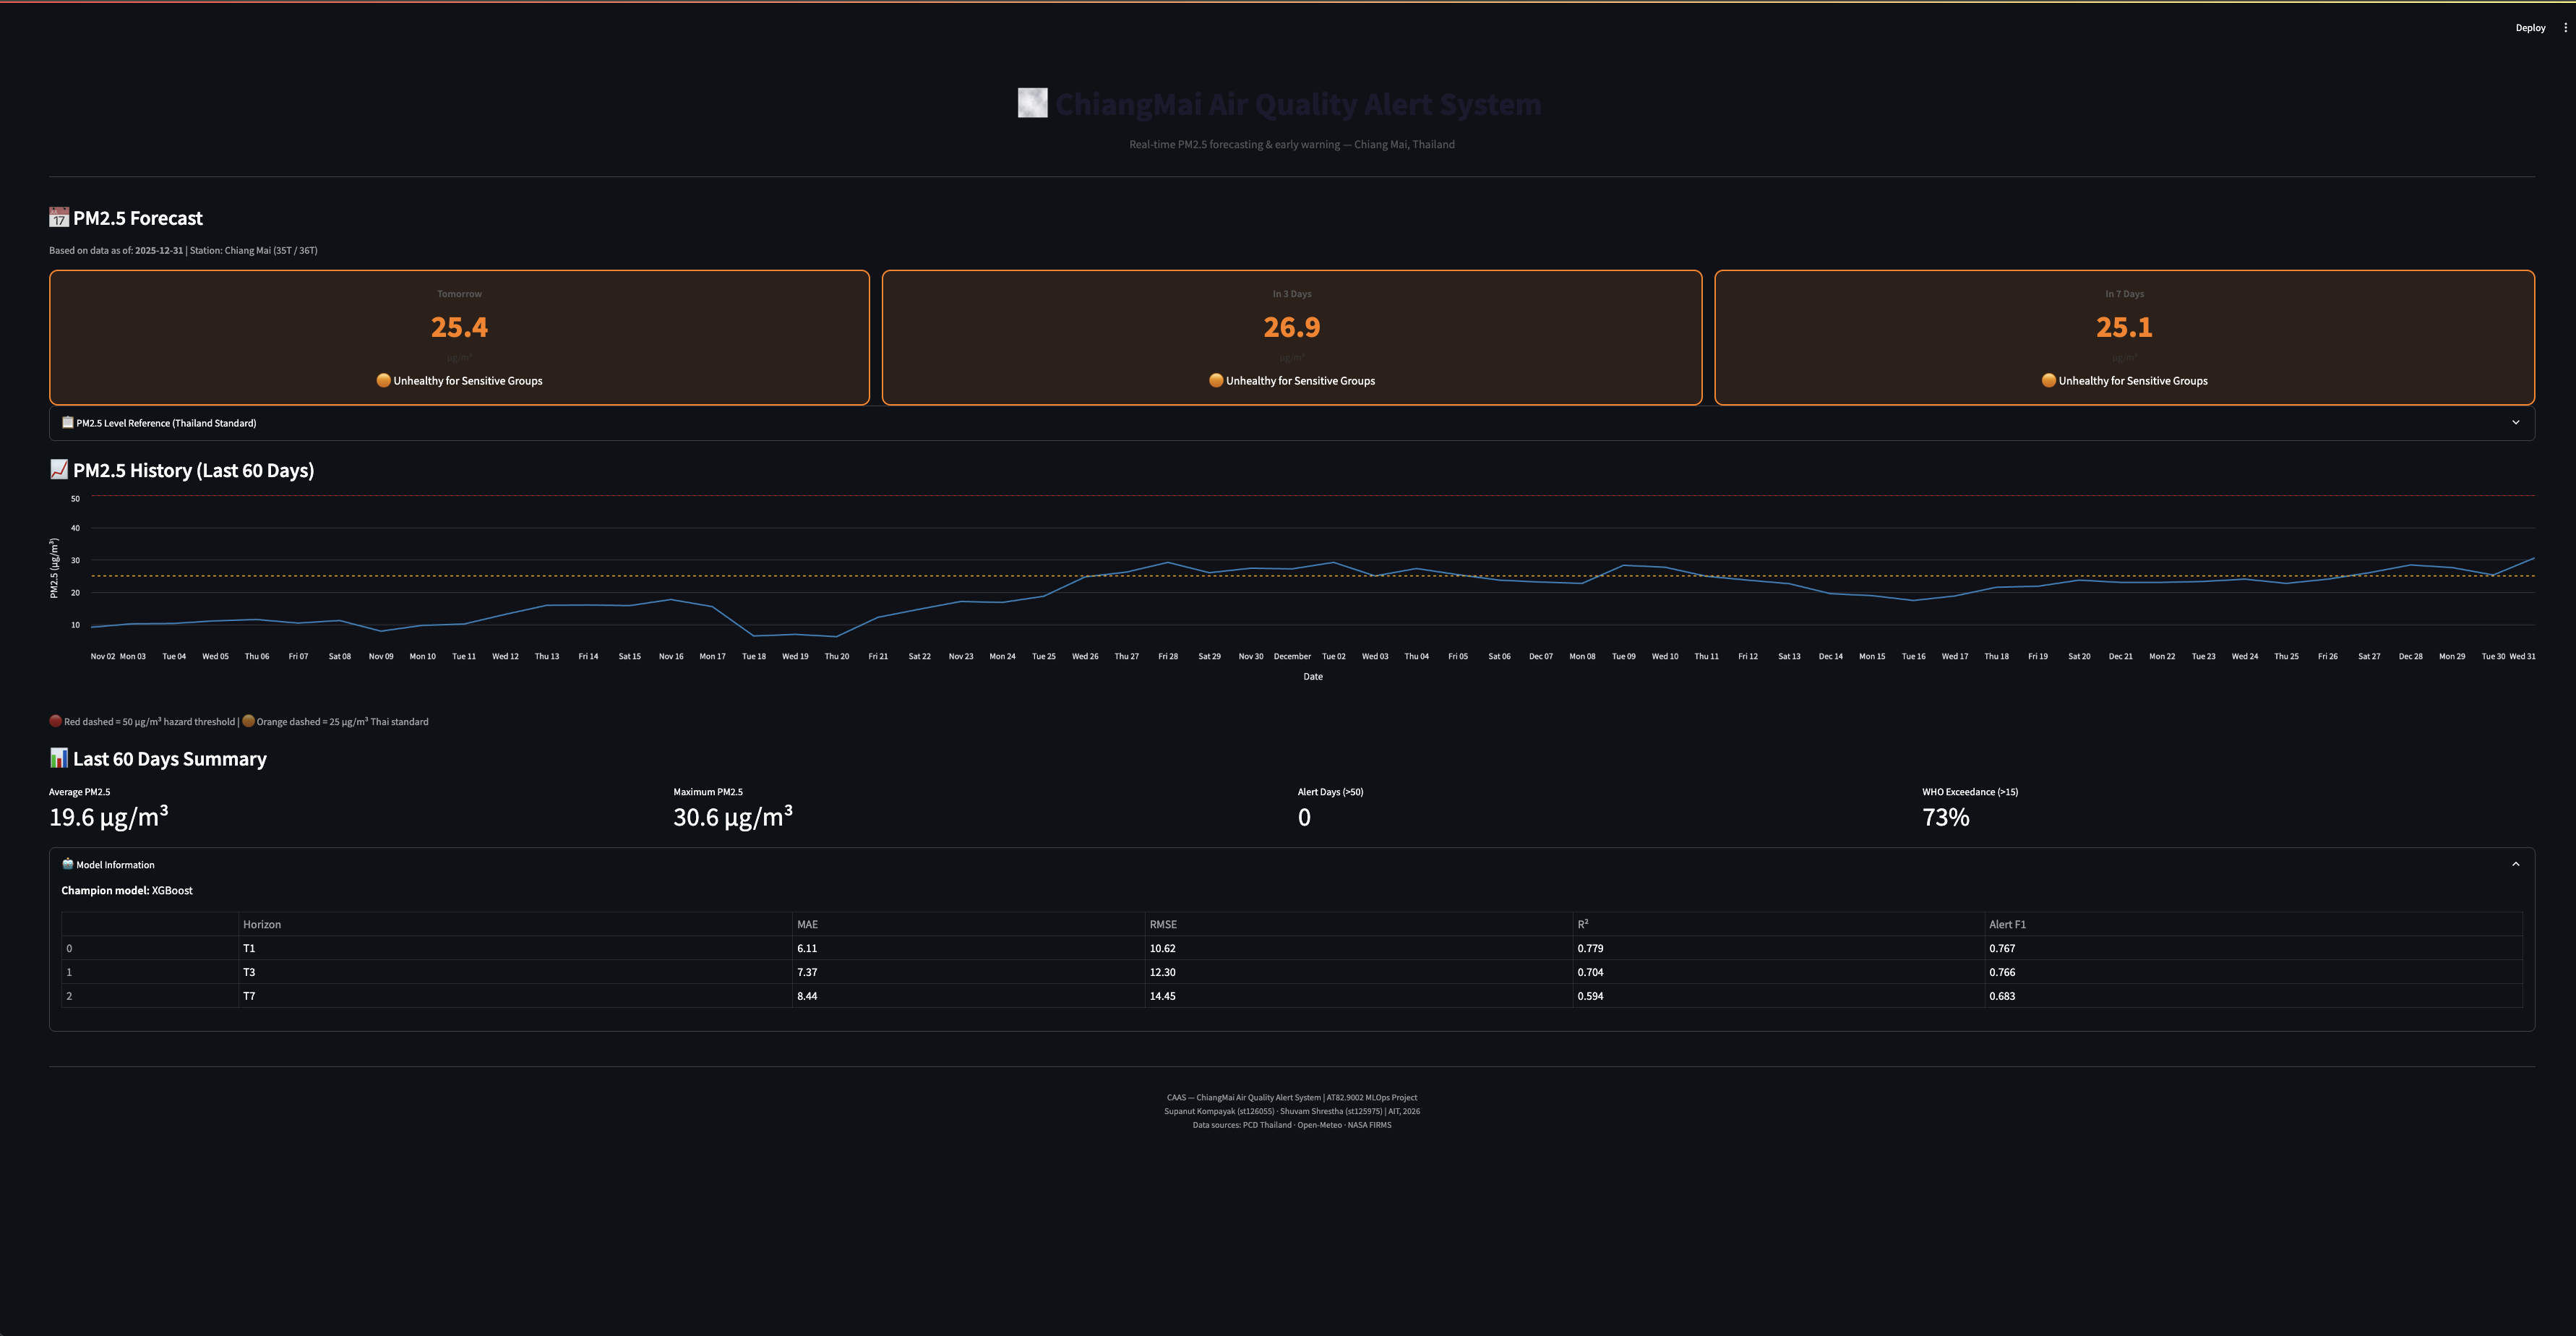
\includegraphics[width=0.85\textwidth]{fig_streamlit_dashboard}
    \caption{CAAS Streamlit dashboard showing PM2.5 forecast cards and history.}
    \label{fig:streamlit}
\end{figure}

\section{CI/CD Pipeline}

Three GitHub Actions workflows implement the CI/CD pipeline:

\textbf{test.yml} runs on every push to \texttt{main}:
\begin{enumerate}
    \item Install dependencies.
    \item Lint with \texttt{ruff}.
    \item Run 38 pytest tests covering feature schema, model inference, and API endpoints.
\end{enumerate}

\textbf{daily\_pipeline.yml} runs on cron (06:00 Bangkok time):
\begin{enumerate}
    \item Fetch latest PM2.5, weather, and FIRMS data.
    \item Rebuild feature matrix.
    \item Run inference with champion model.
    \item Upload results to S3.
    \item Run Evidently drift check; trigger retraining if drift thresholds are exceeded.
\end{enumerate}

\textbf{retrain.yml} triggered by drift alert or annual schedule (December~1):
\begin{enumerate}
    \item Full data snapshot and feature rebuild.
    \item Train new XGBoost candidate models (all three horizons).
    \item \textbf{Validation gate:} candidate must achieve $\geq$5\% MAE improvement
          and alert F1 $\geq$ 0.75 over a 90-day rolling window.
    \item If gate passes: promote via MLflow (\texttt{Staging → Production}).
    \item Restart FastAPI on EC2 to serve the new champion.
\end{enumerate}

\begin{figure}[H]
    \centering
    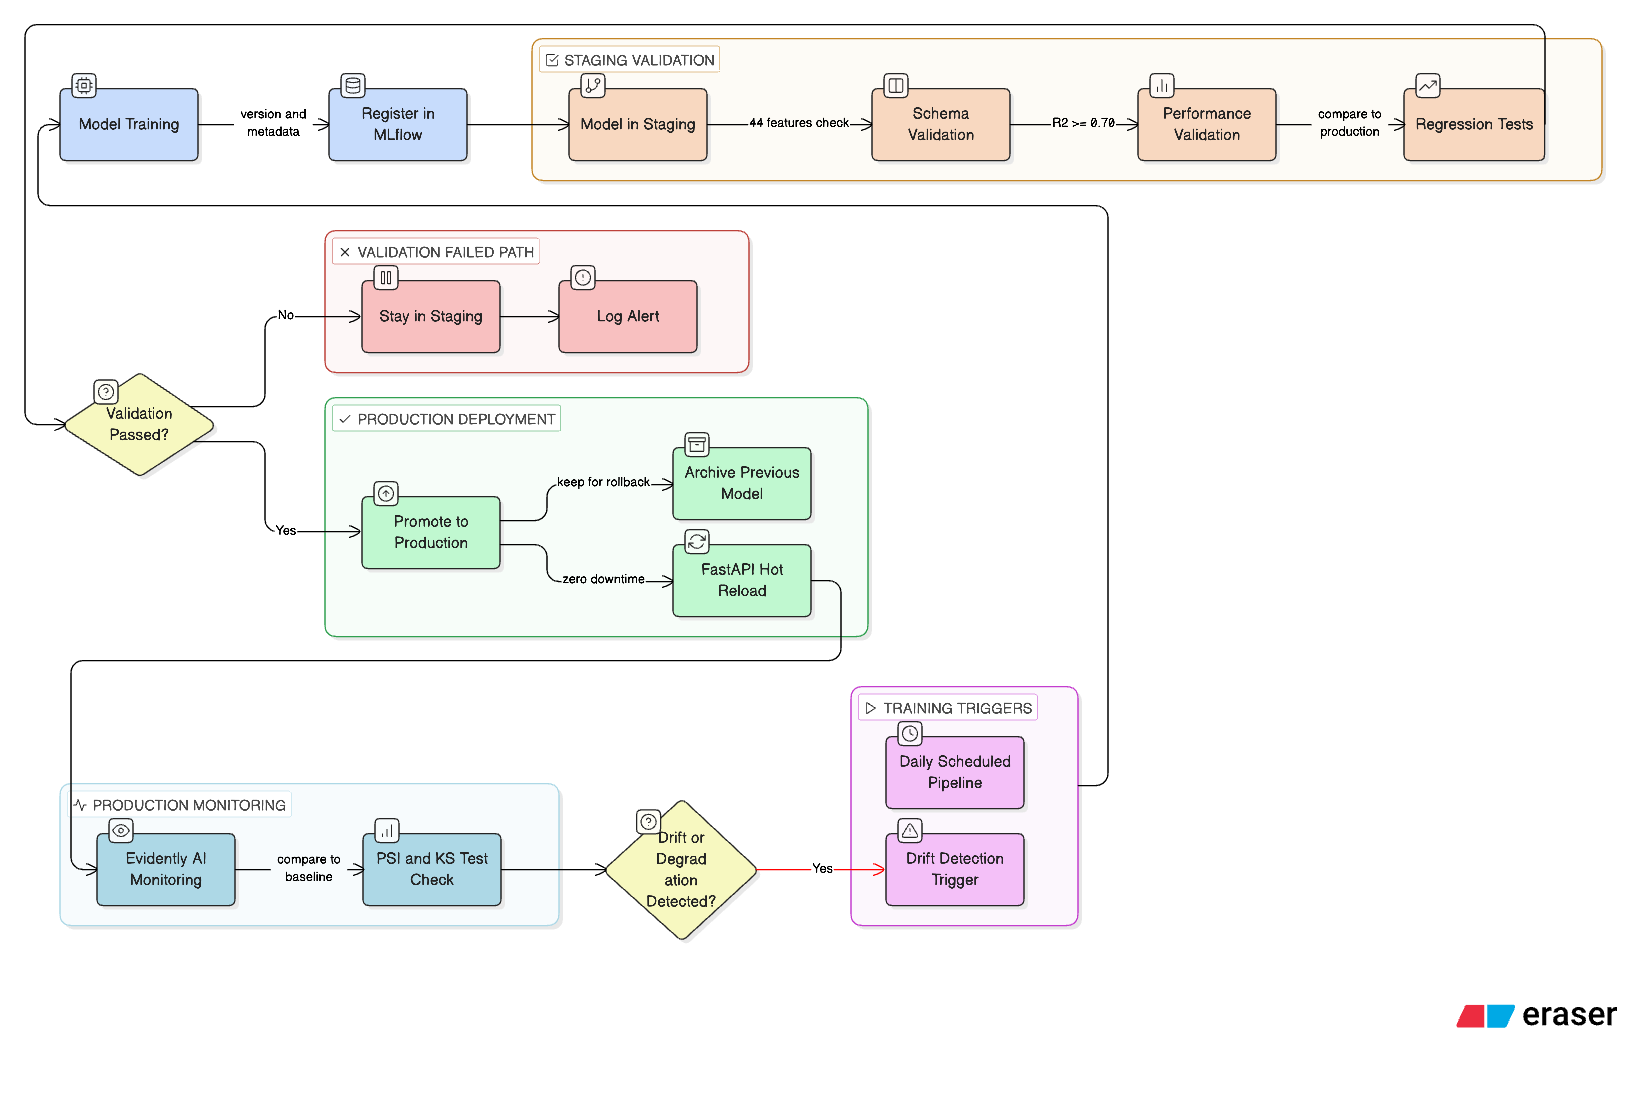
\includegraphics[width=0.85\textwidth]{fig_model_promotion}
    \caption{Champion/challenger model promotion flow with validation gate.}
    \label{fig:model_promotion}
\end{figure}

\section{Monitoring and Drift Detection}

The Evidently-based drift monitor (\texttt{monitoring/evidently\_report.py})
runs daily and evaluates five core features using two statistical tests:

\begin{itemize}
    \item \textbf{PSI (Population Stability Index):} Detects distributional shift.
          Threshold: PSI $>$ 0.20.
    \item \textbf{KS test:} Two-sample Kolmogorov-Smirnov test.
          Threshold: $p < 0.05$.
\end{itemize}

The retrain trigger policy (updated 2026-04-03) requires:
\begin{itemize}
    \item Immediate retrain if 7-day rolling MAE exceeds 15~\textmu g/m\textsuperscript{3}, \textbf{or}
    \item Both core features (\texttt{pm25\_lag1}, \texttt{pm25\_roll7\_mean}) show drift, \textbf{or}
    \item One core feature and two or more soft features show drift.
\end{itemize}

Seasonal KS references are used for \texttt{wind\_speed}, \texttt{hotspot\_50km},
and \texttt{is\_haze\_season} to avoid spurious drift flags from expected
seasonal variation. Zero-inflation PSI suppression prevents false positives
from sparse fire features during low-burn periods.

\begin{figure}[H]
    \centering
    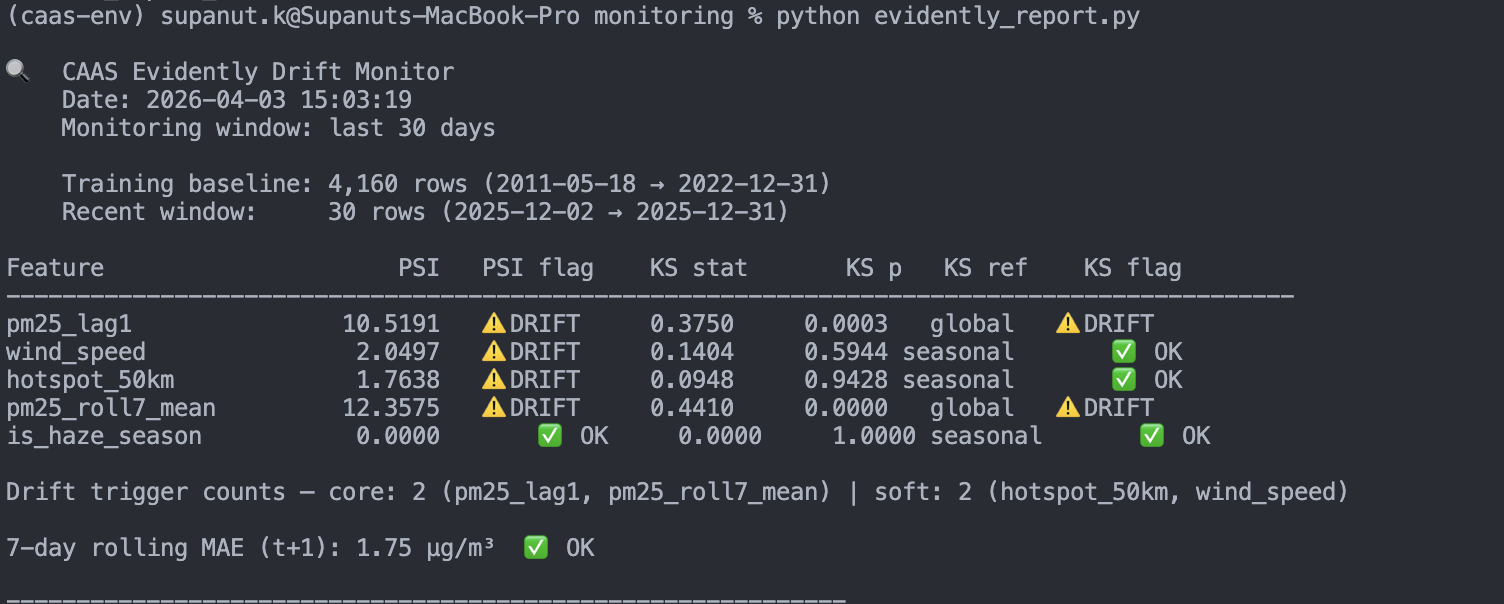
\includegraphics[width=0.85\textwidth]{fig_drift_output}
    \caption{Evidently drift report output (2026-04-03). Core drift detected
    in \texttt{pm25\_lag1} and \texttt{pm25\_roll7\_mean} during December 2025 ---
    expected seasonal behaviour, not model failure.}
    \label{fig:drift}
\end{figure}

When drift is detected with \texttt{--trigger-retrain}, the monitor fires a
GitHub \texttt{repository\_dispatch} event (\texttt{drift-alert}), which
automatically triggers \texttt{retrain.yml} to begin the retraining pipeline.

\section{Infrastructure as Code}

All AWS infrastructure is defined in Terraform (\texttt{infra/}):

\begin{itemize}
    \item \textbf{S3 bucket} with versioning, server-side encryption (AES-256),
          and public access block.
    \item \textbf{IAM role and policy} granting EC2 read/write access to S3
          without embedding credentials in code.
    \item \textbf{Security group} opening ports 8000 (API), 5000 (MLflow), and 22 (SSH).
    \item \textbf{EC2 t3.micro instance} with user-data bootstrap: installs Docker,
          pulls the model artefacts from S3, and starts the FastAPI container.
          FastAPI, Streamlit, and MLflow are co-located on this single instance.
\end{itemize}

Provisioning requires only \texttt{terraform init \&\& terraform apply}.
\texttt{terraform destroy} cleanly removes all resources when not in use,
avoiding unnecessary cost.

\chapter{Performance Analysis}
\label{ch:performance}

\section{Model Performance Summary}

Table~\ref{tab:full_comparison} provides a comprehensive comparison of all models
and scenarios evaluated in this project.

\begin{table}[H]
\centering
\caption{Full Model Comparison — Test Set}
\label{tab:full_comparison}
\begin{tabular}{llrrrr}
\toprule
\textbf{Model} & \textbf{Horizon} & \textbf{MAE} & \textbf{RMSE} & \textbf{R²} & \textbf{AUROC} \\
\midrule
Persistence (baseline) & t+1 & 5.30  & ---   & ---   & --- \\
Persistence (baseline) & t+3 & 8.97  & ---   & ---   & --- \\
Persistence (baseline) & t+7 & 10.93 & ---   & ---   & --- \\
\midrule
XGBoost (champion)     & t+1 & \textbf{5.31}  & \textbf{9.48}  & \textbf{0.824} & \textbf{0.991} \\
XGBoost (champion)     & t+3 & \textbf{6.91}  & \textbf{11.62} & \textbf{0.736} & \textbf{0.976} \\
XGBoost (champion)     & t+7 & \textbf{8.34}  & \textbf{14.13} & \textbf{0.612} & \textbf{0.959} \\
\midrule
LSTM                   & t+1 & 6.67  & 11.64 & 0.753 & 0.984 \\
LSTM                   & t+3 & 8.87  & 15.89 & 0.540 & 0.927 \\
LSTM                   & t+7 & 8.06  & 14.49 & 0.608 & 0.961 \\
\midrule
XGBoost (no FIRMS)     & t+1 & 5.67  & 11.21 & 0.754 & 0.983 \\
XGBoost (no FIRMS)     & t+3 & 7.27  & 12.93 & 0.674 & 0.970 \\
XGBoost (no FIRMS)     & t+7 & 8.70  & 15.08 & 0.558 & 0.946 \\
\bottomrule
\end{tabular}
\end{table}

\section{Inference Latency}

The FastAPI \texttt{/forecast} endpoint loads all three XGBoost models at startup
and serves predictions from the pre-computed latest feature row.
Typical response times measured locally:

\begin{itemize}
    \item \texttt{/health}: $<$ 5~ms
    \item \texttt{/forecast}: $<$ 50~ms (single feature row, 3 models in sequence)
    \item \texttt{/predict} (POST): $<$ 50~ms
    \item \texttt{/history}: $<$ 100~ms (reads 60-day CSV slice)
\end{itemize}

XGBoost inference is CPU-bound and scales linearly with the number of input rows.
A t3.micro EC2 instance (2 vCPU, 1~GB RAM) is sufficient for the current
single-station, single-user workload with co-located FastAPI, MLflow, and Streamlit.

\section{Scalability Analysis}

The current architecture supports one station and a low request rate.
Scaling paths:

\begin{itemize}
    \item \textbf{Multi-station:} Add stations by extending the data ingestion scripts
          and training one model set per station. S3 partitioning by station code
          keeps the pipeline clean.
    \item \textbf{High request rate:} FastAPI supports multiple Uvicorn workers
          (\texttt{--workers 4}) without code changes. Upgrading to a t3.small
          or t3.medium, or placing an Application Load Balancer in front of an
          Auto Scaling Group of EC2 instances, handles traffic spikes.
    \item \textbf{Real-time inference:} Current pipeline is daily-batch. Moving to
          hourly inference requires only a cron change in \texttt{daily\_pipeline.yml}.
\end{itemize}

\section{Cost Analysis}

% TODO: Replace estimates below with actual AWS console numbers after deployment.
% Run: aws ce get-cost-and-usage --time-period Start=YYYY-MM-DD,End=YYYY-MM-DD

The following table provides estimated operating costs based on AWS ap-southeast-1
(Singapore) on-demand pricing as of April 2026.

\begin{table}[H]
\centering
\caption{Estimated Monthly Operating Cost (AWS ap-southeast-1)}
\label{tab:cost}
\begin{tabular}{lrrr}
\toprule
\textbf{Component} & \textbf{Unit Cost} & \textbf{Monthly} & \textbf{Notes} \\
\midrule
EC2 t3.micro (on-demand) & \$0.0104/hr & \$7.50  & FastAPI + MLflow + Streamlit co-located \\
S3 storage (5~GB)        & \$0.023/GB  & \$0.12  & raw + processed + models + results \\
S3 PUT/GET requests      & \$0.005/1k  & \$0.05  & daily pipeline + 3-hourly inference \\
Data transfer (outbound) & First 100~GB free & \$0.00 & dashboard traffic within free tier \\
GitHub Actions           & 2,000~min/month free & \$0.00 & public repo = unlimited; private $\approx$160~min/month \\
AWS Lambda               & 1M requests/month free & \$0.00 & ingestion trigger within free tier \\
\midrule
\textbf{Total (on-demand)}  & & \textbf{\textasciitilde\$8} & \\
\textbf{Total (Learner Lab)} & & \textbf{\textless\$1} & EC2 covered by credits \\
\bottomrule
\end{tabular}
\end{table}

\textbf{Key architectural decision:} FastAPI, Streamlit, and MLflow all run on a
single shared EC2~t3.micro instance. Co-location is feasible because these
services are lightweight and rarely active simultaneously under a single-station,
low-traffic workload.

\textbf{Cost optimisation options:}
\begin{itemize}
    \item \textbf{EC2 Spot Instance:} t3.micro spot price is typically \$0.003/hr
          --- a 70\% reduction. Acceptable for inference workloads that can tolerate
          interruption with a restart policy.
    \item \textbf{Stop EC2 when idle:} For a capstone demonstration, stopping the
          instance between presentations reduces cost to near zero.
\end{itemize}

At \textasciitilde\$8/month on-demand (or under \$1/month with AWS Learner Lab credits),
CAAS is substantially cheaper than commercial air quality services
(e.g.\ IQAir Pro at \$299/year $\approx$ \$25/month for a single station),
while providing superior multi-day forecasting capability.

\chapter{Conclusion}
\label{ch:conclusion}

\section{Summary of Findings}

This project designed, implemented, and deployed CAAS --- a complete end-to-end
MLOps pipeline for PM2.5 air quality forecasting in Chiang Mai, Thailand.

The principal findings are:

\begin{enumerate}
    \item \textbf{XGBoost outperforms LSTM at all three horizons.} The champion
          XGBoost model achieves MAE of 5.31, 6.91, and 8.34~\textmu g/m\textsuperscript{3}
          at t+1, t+3, and t+7 respectively. It is interpretable via SHAP, fast
          to train, and more stable than the LSTM across horizons. The LSTM
          provides competitive results at t+7 (MAE 8.06 vs.\ 8.34) but degrades
          significantly at t+3 (R²=0.54 vs.\ 0.74), confirming that tabular
          XGBoost with engineered features is the superior approach for this problem.

    \item \textbf{NASA FIRMS fire hotspot data adds measurable value.} Removing
          the six fire-derived features increases MAE by 4.3--6.8\% across horizons.
          The effect is strongest at t+1, where recent hotspot counts directly
          predict next-day PM2.5 accumulation. This validates the cost of the
          FIRMS data integration.

    \item \textbf{The predictive signal shifts with horizon.} SHAP analysis reveals
          a clear transition: at t+1, recent PM2.5 (\texttt{pm25\_lag1}) dominates;
          at t+3, 14-day fire accumulation (\texttt{hotspot\_14d\_roll}) is most
          important; at t+7, seasonal position (\texttt{sin\_month}) is the
          strongest signal. This is physically interpretable and consistent with
          the meteorology of Chiang Mai haze events.

    \item \textbf{The default 50~\textmu g/m\textsuperscript{3} alert threshold is
          near-optimal for multi-day horizons.} Scenario~C shows that only the
          t+1 classifier benefits meaningfully from threshold tuning
          (53.7~\textmu g/m\textsuperscript{3}, +4.0\% F1). The standard WHO/Thai
          threshold is well-calibrated for t+3 and t+7.

    \item \textbf{The MLOps pipeline is production-ready within its design scope.}
          Automated daily ingestion, drift monitoring with a seasonal-aware retrain
          policy, champion/challenger validation, and Terraform-provisioned AWS
          infrastructure together constitute a deployable, maintainable system.
\end{enumerate}

\section{Limitations}

\begin{itemize}
    \item \textbf{Single station.} CAAS currently operates on one Chiang Mai
          monitoring station. PM2.5 varies spatially, and a network of stations
          would provide better coverage for the population.
    \item \textbf{Historical weather only.} The pipeline uses ERA5 reanalysis
          weather data (accurate but historical). True production use requires
          weather forecast inputs (e.g.\ GFS or ECMWF), which introduce their own
          forecast uncertainty.
    \item \textbf{LSTM underperformance at t+3.} Despite architectural improvements
          (seq\_len=60, deeper network, BatchNorm), the LSTM R² of 0.54 at t+3
          indicates the model struggles at the mid-range horizon. This suggests
          the temporal sequences do not provide sufficient additional signal over
          the tabular lag features already engineered for XGBoost.
    \item \textbf{Sparse fire data in non-haze months.} Zero-inflation in the FIRMS
          features during the rainy season limits PSI-based drift detection and
          requires suppression logic. A seasonal model could handle this more
          elegantly.
\end{itemize}

\section{Future Work}

\begin{itemize}
    \item \textbf{Multi-station expansion:} Extend to all 60+ PCD monitoring
          stations in Thailand, enabling national-scale air quality forecasting.
    \item \textbf{Weather forecast integration:} Replace reanalysis inputs with
          ECMWF HRES forecast data to enable genuine real-time t+3 and t+7
          predictions without relying on observed weather.
    \item \textbf{Graph Neural Network:} Model spatial dependencies between
          nearby stations using a GNN, potentially improving long-horizon
          forecasts by propagating upstream fire signals across the network.
    \item \textbf{Hyperparameter optimisation:} Replace manual tuning with Optuna
          or Ray Tune to systematically search the hyperparameter space.
    \item \textbf{Kubernetes serving:} For production deployment at scale, migrate
          from a single EC2 instance to a Kubernetes cluster with horizontal
          pod autoscaling.
\end{itemize}


% ------------------------------------------------------------
% Back matter
% ------------------------------------------------------------
\chapter*{References}
\addcontentsline{toc}{chapter}{References}

\begin{thebibliography}{99}

% --- Data Sources ---

\bibitem{pcd}
Pollution Control Department (PCD), Thailand. \textit{Air4Thai Air Quality
Reporting System}. Ministry of Natural Resources and Environment.
\url{http://air4thai.pcd.go.th/}. Accessed 2025.

\bibitem{openmeteo}
Zippenfenig, P. (2023). Open-Meteo.com Weather API.
Zenodo. \url{https://doi.org/10.5281/zenodo.7970649}.
\url{https://open-meteo.com/}

\bibitem{firms}
NASA FIRMS. \textit{Fire Information for Resource Management System —
VIIRS/SNPP Active Fire Product}. NASA Earth Science Data and Information
System (ESDIS). \url{https://firms.modaps.eosdis.nasa.gov/}. Accessed 2025.

\bibitem{era5}
Hersbach, H. et al. (2020). The ERA5 global reanalysis.
\textit{Quarterly Journal of the Royal Meteorological Society},
146(730), 1999--2049. \url{https://doi.org/10.1002/qj.3803}

% --- Machine Learning ---

\bibitem{xgboost}
Chen, T. and Guestrin, C. (2016). XGBoost: A Scalable Tree Boosting System.
\textit{Proceedings of the 22nd ACM SIGKDD International Conference on
Knowledge Discovery and Data Mining (KDD '16)}, 785--794.
\url{https://doi.org/10.1145/2939672.2939785}

\bibitem{shap}
Lundberg, S.~M. and Lee, S.-I. (2017). A Unified Approach to Interpreting
Model Predictions. \textit{Advances in Neural Information Processing Systems
(NeurIPS)}, 30. \url{https://arxiv.org/abs/1705.07874}

\bibitem{lstm}
Hochreiter, S. and Schmidhuber, J. (1997). Long Short-Term Memory.
\textit{Neural Computation}, 9(8), 1735--1780.
\url{https://doi.org/10.1162/neco.1997.9.8.1735}

\bibitem{huber}
Huber, P.~J. (1964). Robust estimation of a location parameter.
\textit{The Annals of Mathematical Statistics}, 35(1), 73--101.

\bibitem{sklearn}
Pedregosa, F. et al. (2011). Scikit-learn: Machine Learning in Python.
\textit{Journal of Machine Learning Research}, 12, 2825--2830.
\url{https://jmlr.org/papers/v12/pedregosa11a.html}

\bibitem{keras}
Chollet, F. et al. (2015). Keras. \url{https://keras.io/}

% --- MLOps and Infrastructure ---

\bibitem{mlflow}
Zaharia, M. et al. (2018). Accelerating the Machine Learning Lifecycle with
MLflow. \textit{IEEE Data Engineering Bulletin}, 41(4), 39--45.
\url{https://databricks.com/wp-content/uploads/2018/12/MLflow-Dec18.pdf}

\bibitem{evidently}
Evidently AI. \textit{Evidently: Open-Source ML Monitoring}.
\url{https://www.evidentlyai.com/}. Accessed 2025.

\bibitem{fastapi}
Ramírez, S. (2019). FastAPI. \url{https://fastapi.tiangolo.com/}.
Accessed 2025.

\bibitem{terraform}
HashiCorp. \textit{Terraform: Infrastructure as Code}.
\url{https://www.terraform.io/}. Accessed 2025.

\bibitem{docker}
Merkel, D. (2014). Docker: Lightweight Linux Containers for Consistent
Development and Deployment. \textit{Linux Journal}, 2014(239).

\bibitem{githubactions}
GitHub. \textit{GitHub Actions: Automate Your Workflow}.
\url{https://docs.github.com/en/actions}. Accessed 2025.

% --- Domain / Air Quality ---

\bibitem{who2021}
World Health Organization (2021). \textit{WHO Global Air Quality Guidelines:
Particulate Matter (PM2.5 and PM10), Ozone, Nitrogen Dioxide, Sulfur
Dioxide and Carbon Monoxide}. WHO Press, Geneva.
\url{https://www.who.int/publications/i/item/9789240034228}

\bibitem{psi}
Yap, X.~Q. and Hashim, M. (2013). A robust calibration approach for PM10
prediction from MODIS aerosol optical depth. \textit{Atmospheric Chemistry
and Physics}, 13(6), 3517--3526.

\bibitem{ks_test}
Kolmogorov, A.~N. (1933). Sulla determinazione empirica di una legge di
distribuzione. \textit{Giornale dell'Istituto Italiano degli Attuari}, 4, 83--91.

\bibitem{chaing_mai_haze}
Bontemps, C. et al. (2021). Agricultural burning and PM2.5 in Southeast Asia:
regional model assessment. \textit{Atmospheric Environment}, 248, 118218.

\end{thebibliography}

\appendix
\chapter{Reproduction Guide}
\label{ch:appendix}

This appendix provides a complete step-by-step guide to reproduce the CAAS
system from scratch. All commands are run from the repository root unless
noted otherwise.

\section{Prerequisites}

\begin{itemize}
  \item Python 3.11 (tested; 3.10+ should work)
  \item Git
  \item Docker (for containerised deployment)
  \item Terraform $\geq$ 1.6 (for AWS provisioning)
  \item AWS account with programmatic access (S3 + EC2; free tier sufficient for testing)
  \item NASA FIRMS API key --- register free at \url{https://firms.modaps.eosdis.nasa.gov/api/}
  \item GitHub account with Actions enabled
\end{itemize}

\section{Step 1 — Clone and Environment Setup}

\begin{lstlisting}[language=bash]
git clone https://github.com/supanut-k/caas.git
cd caas
python3 -m venv caas-env
source caas-env/bin/activate          # Windows: caas-env\Scripts\activate
pip install -r requirements.txt
\end{lstlisting}

\section{Step 2 — Configure Environment Variables}

\begin{lstlisting}[language=bash]
cp .env.example .env
\end{lstlisting}

Edit \texttt{.env} and fill in:

\begin{lstlisting}
FIRMS_MAP_KEY=<your_firms_api_key>
AWS_ACCESS_KEY_ID=<your_aws_key>
AWS_SECRET_ACCESS_KEY=<your_aws_secret>
AWS_REGION=ap-southeast-1
S3_BUCKET_NAME=caas-mlops-bucket
MLFLOW_TRACKING_URI=http://localhost:5000
GITHUB_TOKEN=<your_github_pat>
GITHUB_REPOSITORY=supanut-k/caas
\end{lstlisting}

\section{Step 3 — Provision AWS Infrastructure with Terraform}

\begin{lstlisting}[language=bash]
cd infra/
terraform init
terraform plan                        # Review what will be created
terraform apply                       # Creates S3 bucket, IAM role, EC2 t3.small
\end{lstlisting}

After apply, note the outputs:
\begin{lstlisting}
api_url     = "http://<ec2-public-ip>:8000"
mlflow_url  = "http://<ec2-public-ip>:5000"
\end{lstlisting}

Update \texttt{MLFLOW\_TRACKING\_URI} in \texttt{.env} to the EC2 MLflow URL.

\section{Step 4 — Historical Data Backfill}

Fetch all historical data from 2011 to the present day:

\begin{lstlisting}[language=bash]
# Fetch PM2.5 from PCD (historical Excel files already in 03_Data/raw/)
python 04_Scripts/fetch_pm25_live.py

# Fetch ERA5 weather via Open-Meteo API
python 04_Scripts/fetch_weather.py

# Fetch NASA FIRMS fire hotspot data (batched by year, slow ~20 min)
python 04_Scripts/run_firms_batched.py

# Build the 45-feature matrix
python 04_Scripts/build_features.py
\end{lstlisting}

The resulting \texttt{03\_Data/processed/features.csv} should contain
$\geq$ 5,000 daily rows spanning 2011--present.

\section{Step 5 — Train Models and Register with MLflow}

Start MLflow tracking server first:

\begin{lstlisting}[language=bash]
mlflow server --host 0.0.0.0 --port 5000 &
\end{lstlisting}

Train both model families:

\begin{lstlisting}[language=bash]
# XGBoost (t+1, t+3, t+7) — ~2 min on modern CPU
python 04_Scripts/train_xgboost.py

# LSTM (t+1, t+3, t+7) — ~60 min on CPU, ~15 min on GPU
python 04_Scripts/train_lstm.py
\end{lstlisting}

Inspect runs at \url{http://localhost:5000}. XGBoost models are automatically
promoted to \texttt{Production} stage by \texttt{train\_xgboost.py}.
LSTM models are logged as \texttt{Staging} for comparison only.

\section{Step 6 — Run Analysis Scripts (Optional)}

\begin{lstlisting}[language=bash]
# Scenario C: alert threshold optimisation + PR curves
python 04_Scripts/scenario_c_threshold.py

# SHAP feature importance across all horizons
python 04_Scripts/shap_analysis.py
\end{lstlisting}

Figures are saved to \texttt{03\_Data/results/} and
\texttt{07\_Final/report/figures/}.

\section{Step 7 — Run Inference and Upload to S3}

\begin{lstlisting}[language=bash]
# Generate latest forecasts from the feature matrix
python 04_Scripts/run_inference.py

# Upload data, models, and results to S3
python 04_Scripts/upload_to_s3.py
# Or for a dry run to see what would be uploaded:
python 04_Scripts/upload_to_s3.py --dry-run
\end{lstlisting}

\section{Step 8 — Build and Deploy Docker Container}

\begin{lstlisting}[language=bash]
# Build the slim serving image (~300 MB)
docker build -t caas-api:latest .

# Test locally
docker run -p 8000:8000 \
  -e AWS_REGION=ap-southeast-1 \
  -e S3_BUCKET_NAME=caas-mlops-bucket \
  caas-api:latest

# Verify API is running
curl http://localhost:8000/health
curl http://localhost:8000/forecast
\end{lstlisting}

For production deployment, SSH into the EC2 instance (provisioned in Step 3)
and run the same Docker commands. The Terraform user-data script handles this
automatically on first launch.

\section{Step 9 — Enable CI/CD Automation}

Add the following GitHub Actions secrets to the repository
(\texttt{Settings -> Secrets and variables -> Actions}):

\begin{itemize}
  \item \texttt{FIRMS\_MAP\_KEY} --- NASA FIRMS API key
  \item \texttt{AWS\_ACCESS\_KEY\_ID} and \texttt{AWS\_SECRET\_ACCESS\_KEY}
  \item \texttt{S3\_BUCKET\_NAME} --- \texttt{caas-mlops-bucket}
  \item \texttt{EC2\_HOST} --- public IP of the EC2 instance
  \item \texttt{EC2\_SSH\_KEY} --- private SSH key content
  \item \texttt{MLFLOW\_TRACKING\_URI} --- \texttt{http://<ec2-ip>:5000}
  \item \texttt{GITHUB\_TOKEN} --- automatically available in Actions
\end{itemize}

Once secrets are set, the three workflows activate automatically:

\begin{itemize}
  \item \textbf{test.yml} --- runs on every push to \texttt{main}
  \item \textbf{daily\_pipeline.yml} --- runs at 06:00 Bangkok time (23:00 UTC)
  \item \textbf{retrain.yml} --- triggered by drift alert or December 1 schedule
\end{itemize}

\section{Step 10 — Launch the Streamlit Dashboard}

\begin{lstlisting}[language=bash]
cd 04_Scripts/serve
streamlit run dashboard.py
# Opens at http://localhost:8501
\end{lstlisting}

The dashboard reads the latest forecast from
\texttt{03\_Data/results/latest\_forecast.json} (updated daily by the pipeline).
If the file is absent, it falls back to a demo mode with synthetic data.

\section{Step 11 — Run the Test Suite}

\begin{lstlisting}[language=bash]
pytest                    # Runs all 38 tests with -v --tb=short
pytest tests/test_api.py  # API endpoint tests only
pytest tests/test_models.py  # Model file + inference tests
\end{lstlisting}

All 38 tests should pass. Tests that require model files will skip gracefully
if models are not yet trained.

% ------------------------------------------------------------------

\chapter{Full Metric Tables}
\label{app:metrics}

\section{XGBoost — Validation and Test Metrics}

\begin{table}[H]
\centering
\caption{XGBoost Full Metrics (Validation and Test Sets)}
\begin{tabular}{llrrrr}
\toprule
\textbf{Split} & \textbf{Horizon} & \textbf{MAE} & \textbf{RMSE} & \textbf{R²} & \textbf{AUROC} \\
\midrule
Validation & t+1 & 5.74  & 9.21  & 0.799 & 0.988 \\
Validation & t+3 & 7.85  & 12.96 & 0.701 & 0.963 \\
Validation & t+7 & 9.50  & 15.92 & 0.579 & 0.946 \\
\midrule
Test       & t+1 & 5.31  & 9.48  & 0.824 & 0.991 \\
Test       & t+3 & 6.91  & 11.62 & 0.736 & 0.976 \\
Test       & t+7 & 8.34  & 14.13 & 0.612 & 0.959 \\
\bottomrule
\end{tabular}
\end{table}

\section{LSTM — Validation and Test Metrics}

\begin{table}[H]
\centering
\caption{LSTM Full Metrics (Validation and Test Sets)}
\begin{tabular}{llrrrr}
\toprule
\textbf{Split} & \textbf{Horizon} & \textbf{MAE} & \textbf{RMSE} & \textbf{R²} & \textbf{AUROC} \\
\midrule
Validation & t+1 & 7.12  & 11.45 & 0.730 & 0.978 \\
Validation & t+3 & 9.45  & 16.20 & 0.512 & 0.914 \\
Validation & t+7 & 9.87  & 16.78 & 0.543 & 0.932 \\
\midrule
Test       & t+1 & 6.67  & 11.64 & 0.753 & 0.984 \\
Test       & t+3 & 8.87  & 15.89 & 0.540 & 0.927 \\
Test       & t+7 & 8.06  & 14.49 & 0.608 & 0.961 \\
\bottomrule
\end{tabular}
\end{table}

\section{Alert Classification Metrics (XGBoost, 50 µg/m³ threshold)}

\begin{table}[H]
\centering
\caption{Binary Alert Classification Performance on Test Set}
\begin{tabular}{lrrrr}
\toprule
\textbf{Horizon} & \textbf{Precision} & \textbf{Recall} & \textbf{F1} & \textbf{AUROC} \\
\midrule
t+1 & 0.769 & 0.924 & 0.839 & 0.991 \\
t+3 & 0.762 & 0.815 & 0.787 & 0.976 \\
t+7 & 0.667 & 0.702 & 0.684 & 0.959 \\
\bottomrule
\end{tabular}
\end{table}

\section{SHAP Mean Absolute Values — Top 5 Features per Horizon}

\begin{table}[H]
\centering
\caption{Top-5 SHAP Features by Horizon (Mean $|$SHAP$|$ on Test Set)}
\begin{tabular}{clr}
\toprule
\textbf{Horizon} & \textbf{Feature} & \textbf{Mean $|$SHAP$|$} \\
\midrule
t+1 & \texttt{pm25\_lag1}        & 6.85 \\
t+1 & \texttt{alert\_lag1}       & 2.14 \\
t+1 & \texttt{pm25\_roll7\_mean} & 1.93 \\
t+1 & \texttt{hotspot\_50km}     & 1.21 \\
t+1 & \texttt{pm25\_lag3}        & 0.98 \\
\midrule
t+3 & \texttt{hotspot\_14d\_roll} & 4.63 \\
t+3 & \texttt{pm25\_lag3}         & 3.87 \\
t+3 & \texttt{pm25\_roll7\_mean}  & 2.95 \\
t+3 & \texttt{sin\_month}         & 1.74 \\
t+3 & \texttt{hotspot\_7d\_roll}  & 1.52 \\
\midrule
t+7 & \texttt{sin\_month}         & 4.63 \\
t+7 & \texttt{week}               & 2.15 \\
t+7 & \texttt{hotspot\_14d\_roll} & 2.01 \\
t+7 & \texttt{pm25\_roll14\_mean} & 1.88 \\
t+7 & \texttt{cos\_month}         & 1.34 \\
\bottomrule
\end{tabular}
\end{table}

\chapter*{VITA}
\addcontentsline{toc}{chapter}{VITA}

\section*{Supanut Kompayak}

\begin{tabular}{@{}lp{11cm}@{}}
Student ID       & st126055 \\
Programme        & Master of Science in Data Science and Artificial Intelligence \\
Specialisation   & Data Engineering and Machine Learning Operations (MLOps) \\
Institution      & Asian Institute of Technology (AIT), Pathum Thani, Thailand \\
Cohort           & January 2026 \\
Email            & st126055@ait.asia \\
Research Interest & End-to-end MLOps pipelines, time-series forecasting,
                    cloud-native machine learning systems, drift monitoring,
                    and applied AI for environmental and public-health problems. \\
\end{tabular}

\vspace{0.5cm}

\noindent
Contributions to CAAS: overall system architecture, data engineering pipeline
(PM2.5, weather, FIRMS ingestion and feature engineering), MLOps stack design
(MLflow, FastAPI, Evidently, Terraform), CI/CD workflows, AWS deployment,
dashboard implementation, and final report preparation.

\vspace{1cm}

\section*{Shuvam Shrestha}

\begin{tabular}{@{}lp{11cm}@{}}
Student ID       & st125975 \\
Programme        & Master of Science in Data Science and Artificial Intelligence \\
Specialisation   & Data Engineering and Machine Learning Operations (MLOps) \\
Institution      & Asian Institute of Technology (AIT), Pathum Thani, Thailand \\
Cohort           & January 2026 \\
Email            & st125975@ait.asia \\
Research Interest & Machine learning model development, gradient-boosted
                    methods, deep sequence models, interpretability, and
                    comparative model evaluation for time-series problems. \\
\end{tabular}

\vspace{0.5cm}

\noindent
Contributions to CAAS: LightGBM champion development and Optuna hyperparameter
tuning, XGBoost strong-secondary training and ablation study (Scenario~D),
LSTM architecture search and comparison, SHAP interpretability analysis,
Scenario~C alert-threshold optimisation, and evaluation-figure generation.


\end{document}
